%%%%%%%%%%%%%%%%%%%%%%%%%%%%%%%%%%%%%%%%%
% Masters/Doctoral Thesis 
% LaTeX Template
% Version 2.4 (22/11/16)
%
% This template has been downloaded from:
% http://www.LaTeXTemplates.com
%
% Version 2.x major modifications by:
% Vel (vel@latextemplates.com)
%
% This template is based on a template by:
% Steve Gunn (http://users.ecs.soton.ac.uk/srg/softwaretools/document/templates/)
% Sunil Patel (http://www.sunilpatel.co.uk/thesis-template/)
%
% Template license:
% CC BY-NC-SA 3.0 (http://creativecommons.org/licenses/by-nc-sa/3.0/)
%
%%%%%%%%%%%%%%%%%%%%%%%%%%%%%%%%%%%%%%%%%
%----------------------------------------------------------------------------------------
%	PACKAGES AND OTHER DOCUMENT CONFIGURATIONS
%----------------------------------------------------------------------------------------

\documentclass[
12pt, % The default document font size, options: 10pt, 11pt, 12pt
%oneside, % Two side (alternating margins) for binding by default, uncomment to switch to one side
english, % ngerman for German
onehalfspacing, % Single line spacing, alternatives: onehalfspacing or doublespacing
%draft, % Uncomment to enable draft mode (no pictures, no links, overfull hboxes indicated)
%nolistspacing, % If the document is onehalfspacing or doublespacing, uncomment this to set spacing in lists to single
%liststotoc, % Uncomment to add the list of figures/tables/etc to the table of contents
%toctotoc, % Uncomment to add the main table of contents to the table of contents
%parskip, % Uncomment to add space between paragraphs
%nohyperref, % Uncomment to not load the hyperref package
headsepline, % Uncomment to get a line under the header
%chapterinoneline, % Uncomment to place the chapter title next to the number on one line
%consistentlayout, % Uncomment to change the layout of the declaration, abstract and acknowledgements pages to match the default layout
%longbibliography,
]{MastersDoctoralThesis} % The class file specifying the document structure

\usepackage[utf8]{inputenc} % Required for inputting international characters
\usepackage[T1]{fontenc} % Output font encoding for international characters
\usepackage{siunitx}
\usepackage{times} % Use the Palatino font by default
\usepackage{textgreek}
\usepackage{textcomp}
%\usepackage{titlesec}
\usepackage{caption}
\usepackage[calcwidth = \linewidth, labelfont = bf, textfont=bf]{caption}
\usepackage{ragged2e}
\usepackage[section]{placeins}
\usepackage{commath}
\usepackage{subcaption}
%\usepackage{physics}
%\usepackage[backend=bibtex,style=authoryear,natbib=true]{biblatex} % Use the bibtex backend with the authoryear citation style (which resembles APA)

%\addbibresource{main.bib} % The filename of the bibliography

%\usepackage[autostyle=true]{csquotes} % Required to generate language-dependent quotes in the bibliography

\usepackage[sort&compress,numbers]{natbib}
\usepackage{verbatim}
\bibliographystyle{apsrev4-1}
%\usepackage{doi}%<----------
%\usepackage{hyperref}
\def\bibsection{\section*{\refname}} 
\sisetup{detect-all}
\captionsetup{font=normalsize,width=\columnwidth}
%\titleformat*{\section}{\Large\bfseries}
%----------------------------------------------------------------------------------------
%	MARGIN SETTINGS
%----------------------------------------------------------------------------------------

\geometry{
	paper=a4paper, % Change to letterpaper for US letter
	inner=2.5cm, % Inner margin
	outer=2.5cm, % Outer margin
	bindingoffset=.5cm, % Binding offset
	top=2.5cm, % Top margin
	bottom=2.5cm, % Bottom margin
	%showframe, % Uncomment to show how the type block is set on the page
}

%----------------------------------------------------------------------------------------
%	THESIS INFORMATION
%----------------------------------------------------------------------------------------

\thesistitle{Characterizing the Role of a GLUT1 Mutation in GLUT1-deficiency Syndrome} % Your thesis title, this is used in the title and abstract, print it elsewhere with \ttitle
\supervisor{Prof. Dr. Matthias \textsc{Selbach}} % Your supervisor's name, this is used in the title page, print it elsewhere with \supname
\examiner{} % Your examiner's name, this is not currently used anywhere in the template, print it elsewhere with \examname
\degree{Master of Science} % Your degree name, this is used in the title page and abstract, print it elsewhere with \degreename
\author{Jingyuan \textsc{Cheng}} % Your name, this is used in the title page and abstract, print it elsewhere with \authorname
\addresses{} % Your address, this is not currently used anywhere in the template, print it elsewhere with \addressname

\subject{Molecular Medicine} % Your subject area, this is not currently used anywhere in the template, print it elsewhere with \subjectname
\keywords{} % Keywords for your thesis, this is not currently used anywhere in the template, print it elsewhere with \keywordnames
\university{Charit\'{e} Universit\"{a}tsmedizin Berlin} % Your university's name and URL, this is used in the title page and abstract, print it elsewhere with \univname
\department{Protein Dynamics} % Your department's name and URL, this is used in the title page and abstract, print it elsewhere with \deptname
\group{Protein Dynamics} % Your research group's name and URL, this is used in the title page, print it elsewhere with \groupname
\faculty{} % Your faculty's name and URL, this is used in the title page and abstract, print it elsewhere with \facname

\AtBeginDocument{
\hypersetup{pdftitle=\ttitle} % Set the PDF's title to your title
\hypersetup{pdfauthor=\authorname} % Set the PDF's author to your name
\hypersetup{pdfkeywords=\keywordnames} % Set the PDF's keywords to your keywords
}

\begin{document}

\frontmatter % Use roman page numbering style (i, ii, iii, iv...) for the pre-content pages

\pagestyle{plain} % Default to the plain heading style until the thesis style is called for the body content

%----------------------------------------------------------------------------------------
%	TITLE PAGE
%----------------------------------------------------------------------------------------

\begin{titlepage}
\begin{center}

\begin{figure}
\centering

\includegraphics[scale=1.0]{Figures/Charite.pdf}\ \\[2ex]

\Large\bfseries Master's Program in Molecular Medicine\\
\Large at the Charit\'{e} - Universit\"{a}tsmedizin Berlin\\
\vspace*{1cm}

\includegraphics[scale=1.0]{Figures/molmed.pdf}
\label{titlepictures}
\end{figure}

\LARGE\bfseries Master's Thesis\\
\large\normalfont to earn the\\
\LARGE\bfseries Master of Science in Molecular Medicine\\

\vspace*{1cm}

\LARGE\bfseries Characterizing the Role of a GLUT1 Mutation in GLUT1-deficiency Syndrome

\vspace*{1cm}

\large\normalfont Presented by\\
\bfseries Jingyuan Cheng\\
\large\normalfont Born on May 17th, 1993\\

\vspace*{1cm}
\end{center}
\begin{flushleft}
\large\normalfont First Evaluator: Professor Dr. Matthias Selbach\\
Second Evaluator: Professor Dr. Volker Haucke\\

\vspace*{1cm}

Completed at AG Selbach, Max Delbr\"{u}ck Center for Molecular Medicine
\end{flushleft}

\begin{comment}

\vspace*{.06\textheight}
{\scshape\LARGE \univname\par}\vspace{1.5cm} % University name
% \textsc{\Large Doctoral Thesis}\\[0.5cm] % Thesis type

\HRule \\[0.4cm] % Horizontal line
{\huge \bfseries \ttitle\par}\vspace{0.4cm} % Thesis title
\HRule \\[1.5cm] % Horizontal line
 
\begin{minipage}[t]{0.4\textwidth}
\begin{flushleft} \large
\emph{Author:}\\
\authorname % Author name - remove the \href bracket to remove the link
\end{flushleft}
\end{minipage}
\begin{minipage}[t]{0.4\textwidth}
\begin{flushright} \large
\emph{Supervisor:} \supname % Supervisor name - remove the \href bracket to remove the link  
\end{flushright}
\end{minipage}\\[3cm]
 
\vfill

\large \textit{A thesis submitted in fulfillment of the requirements\\ for the degree of \degreename}\\[0.3cm] % University requirement text
\textit{in the}\\[0.4cm]
%\groupname\\\deptname\\[2cm] % Research group name and department name
 
\vfill

{\large \today}\\[4cm] % Date
%\includegraphics{Logo} % University/department logo - uncomment to place it

\end{comment}
 
\vfill
\end{titlepage}

%----------------------------------------------------------------------------------------
%	ABSTRACT PAGE
%----------------------------------------------------------------------------------------

\begin{abstract}
\addchaptertocentry{\abstractname} % Add the abstract to the table of contents
%need modification
Glucose transporter-1 (GLUT1) deficiency syndrome is a genetic disorder characterized by impaired glucose transport into the brain. One of the clinically identified pathogenic mutations is a Pro485-to-Leu substitution located in the cytoplasmic carboxyl tail of GLUT1, whose pathogenic mechanisms remain unclear. A previous \textit{in vitro} proteomic screen from our group revealed that this GLUT1 mutation leads to specific interactions with clathrin, which is supported by the further bioinformatic finding that the mutation creates a novel dileucine motif known to mediate clathrin-dependent trafficking. \\
\\*
In this study we used stable inducible HEK293 cells to further investigate the effect of the GLUT1 mutation on the intracellular localization and trafficking of the protein. We showed that the wild-type GLUT1 mainly localizes to the plasma membrane, whereas the mutant GLUT1 mislocalizes to intracellular compartments and co-localizes with endocytosed transferrin, as well as early endosomal and late endosomal markers. Moreover, SILAC-based quantitative characterization of proximate proteins also identified increased proximate interaction of the mutant GLUT1 with proteins associated with endocytosis and endosomal compartments. Together, these data suggest that the GLUT1\textsuperscript{P485L} mutation causes internalization of the GLUT1 protein via clathrin-mediated endocytosis, thus leading to GLUT1 deficiency syndrome.\\

%On the other hand, the mutant GLUT1 shows no co-localization with the lysosomal marker LAMP1, and the inhibition of lysosomal degradation cannot increase the mutant GLUT1 level. These results suggest that the mutant GLUT1 

\end{abstract}

%----------------------------------------------------------------------------------------
%	LIST OF CONTENTS/FIGURES/TABLES PAGES
%----------------------------------------------------------------------------------------

\tableofcontents % Prints the main table of contents

\listoffigures % Prints the list of figures

\listoftables % Prints the list of tables

%----------------------------------------------------------------------------------------
%	THESIS CONTENT - CHAPTERS
%----------------------------------------------------------------------------------------

\mainmatter % Begin numeric (1,2,3...) page numbering

\pagestyle{thesis} % Return the page headers back to the "thesis" style

% Include the chapters of the thesis as separate files from the Chapters folder
% Uncomment the lines as you write the chapters

% Chapter 1

\chapter{Introduction} % Main chapter title
\label{Chapter1} % For referencing the chapter elsewhere, use \ref{Chapter1} 

%----------------------------------------------------------------------------------------
As the primary glucose transporter across the endothelial cells of the blood-brain barrier, the GLUT1 protein plays a central role in the regulation of brain energy metabolism and maintenance of central nervous system homeostasis~\cite{Pascual}. Human GLUT1 has 492 amino acids, many of which have been reported to be susceptible to missense mutation that causes GLUT1 deficiency syndrome (G1DS), a genetic disease characterized by hypoglycorrhachia (low glucose concentration in the cerebrospinal fluid), seizures and delayed neurological development~\cite{Pascual,De}. GLUT1 mutations in G1DS patients impair glucose transport into the brain across the blood-brain barrier, resulting in the disease phenotypes. 

One of the clinically identified missense mutations in GLUT1 is a Pro485-to-Leu substitution (GLUT1\textsuperscript{P485L}) located in the cytoplasmic carboxyl tail~\cite{Pascual,Slaughter}. However, the molecular mechanisms by which the mutation causes the disease remains elusive. In a previous proteomic screen study to investigate the impact of disease-causing mutations, the GLUT1\textsuperscript{P485L} mutation was found to lead to an increased binding of clathrins. Sequence analysis revealed that the mutation creates a dileucine motif known to mediate clathrin-dependent endocytosis ([D/E]XXXL[L/I]) in the cytoplasmic tail~\cite{Pandey,Dinkel}.
%peptide-based interaction screen on disease-causing mutations

%TPEELFHLLGADSQV
% [D/E]XXXL[L/I] 

%A previous study of the group combined high-throughput peptide pull-downs and quantitative mass spectrometry~\cite{Meyer} to study binding profiles of proteins with disease related mutations. The results have shown that a peptide on the carboxyl terminal of GLUT1 with Pro485-to-Leu mutation (TPEELFHLLGADSQV) binds with clathrin, and this interaction is absent in the binding profile of the wild type peptide. Accordantly, the mutation creates a short linear motif (E...LL) in the cytoplasmic tail region of GLUT1 that interacts with adaptor proteins such as APs and mediates clathrin-dependent endocytic sorting~\cite{Traub}. Furthermore, a proximity-dependent biotin identification (BioID) experiment~\cite{Roux} in HEK293 cells transiently transfected with GLUT1 provides additional evidence for the novel interaction between the mutant GLUT1 and several proteins involved in the clathrin-mediated endocytosis pathway.

Based on these findings, it is hypothesized that the GLUT1\textsuperscript{P485L} mutation causes clathrin-mediated endocytosis and possibly subsequent degradation of GLUT1, leading to the development of GLUT1-deficiency syndrome. The hypothesis will be further investigated in this master thesis.

% Define some commands to keep the formatting separated from the content 
\newcommand{\keyword}[1]{\textbf{#1}}
\newcommand{\tabhead}[1]{\textbf{#1}}
\newcommand{\code}[1]{\texttt{#1}}
\newcommand{\file}[1]{\texttt{\bfseries#1}}
\newcommand{\option}[1]{\texttt{\itshape#1}}



% Chapter 2

\chapter{Materials and methods} % Main chapter title
\label{Chapter2} % For referencing the chapter elsewhere, use \ref{Chapter2}

\bfseries{Cell line generation}\\
\normalfont Doxycycline-inducible wild-type and mutant GLUT1-expressing cell lines had been generated previously in the lab of Markus Landthaler at Max Delbr\"{u}ck Center. In brief, the gene \textit{SLC2A1} was purchased from Harvard Plasmid Repository and a stop codon was added with the primers listed in Table~\ref{tab:primers} (BioTeZ). The P485L mutation was introduced by PCR-directed mutagenesis with the primers listed in Table~\ref{tab:primers}. The wild-type and mutant \textit{SLC2A1} coding sequences were recombined into the vector pDEST-pcDNA5-BirA-FLAG using Gateway cloning system (ThermoFisher) (Figure~\ref{fig:vectors})~\cite{Couzens}. HEK293 Flp-In T-Rex cells (Invitrogen) were cotransfected with pOG44 Flp-recombinase expression vector (ThermoFisher) and the recombinant vector containing wild-type or mutant GLUT1 to generate stable cell lines. Two days following transfection, cells were selected with 100 \textmu g/mL Hygromycin B (InvivoGen) for 2 weeks. A control HEK293 cell line for BioID experiments had been generated in the lab using the identical technique with an integrated transgene for the inducible expression of the first 10 strands of GFP (GFP1-10).

\begin{table}[h]
%\captionsetup{font=normalsize}
\caption{Primer sequences for mutagenesis of GLUT1.}
\label{tab:primers}
\small
\centering
\begin{tabular*}{\textwidth}{l@{\extracolsep{\fill}}p{11.1cm}}
\toprule
\tabhead{Purpose} & \tabhead{Primer sequences (5' to 3')}\\
\midrule
Adding a stop codon & Forward: TCCCAAGTGTAATTGCCAACTTTCTTGTACAAAGTTG \newline Reverse: ATCAGCCCCCAGGGGATG\\
P485L mutation & Forward: CTGTTCCATCTCCTGGGGGCT \newline Reverse: CTCCTCGGGTGTCTTGTCAC\\
\bottomrule\\
\end{tabular*}
\end{table}
\begin{figure}[h]
%\captionsetup{font=normalsize}
\centering
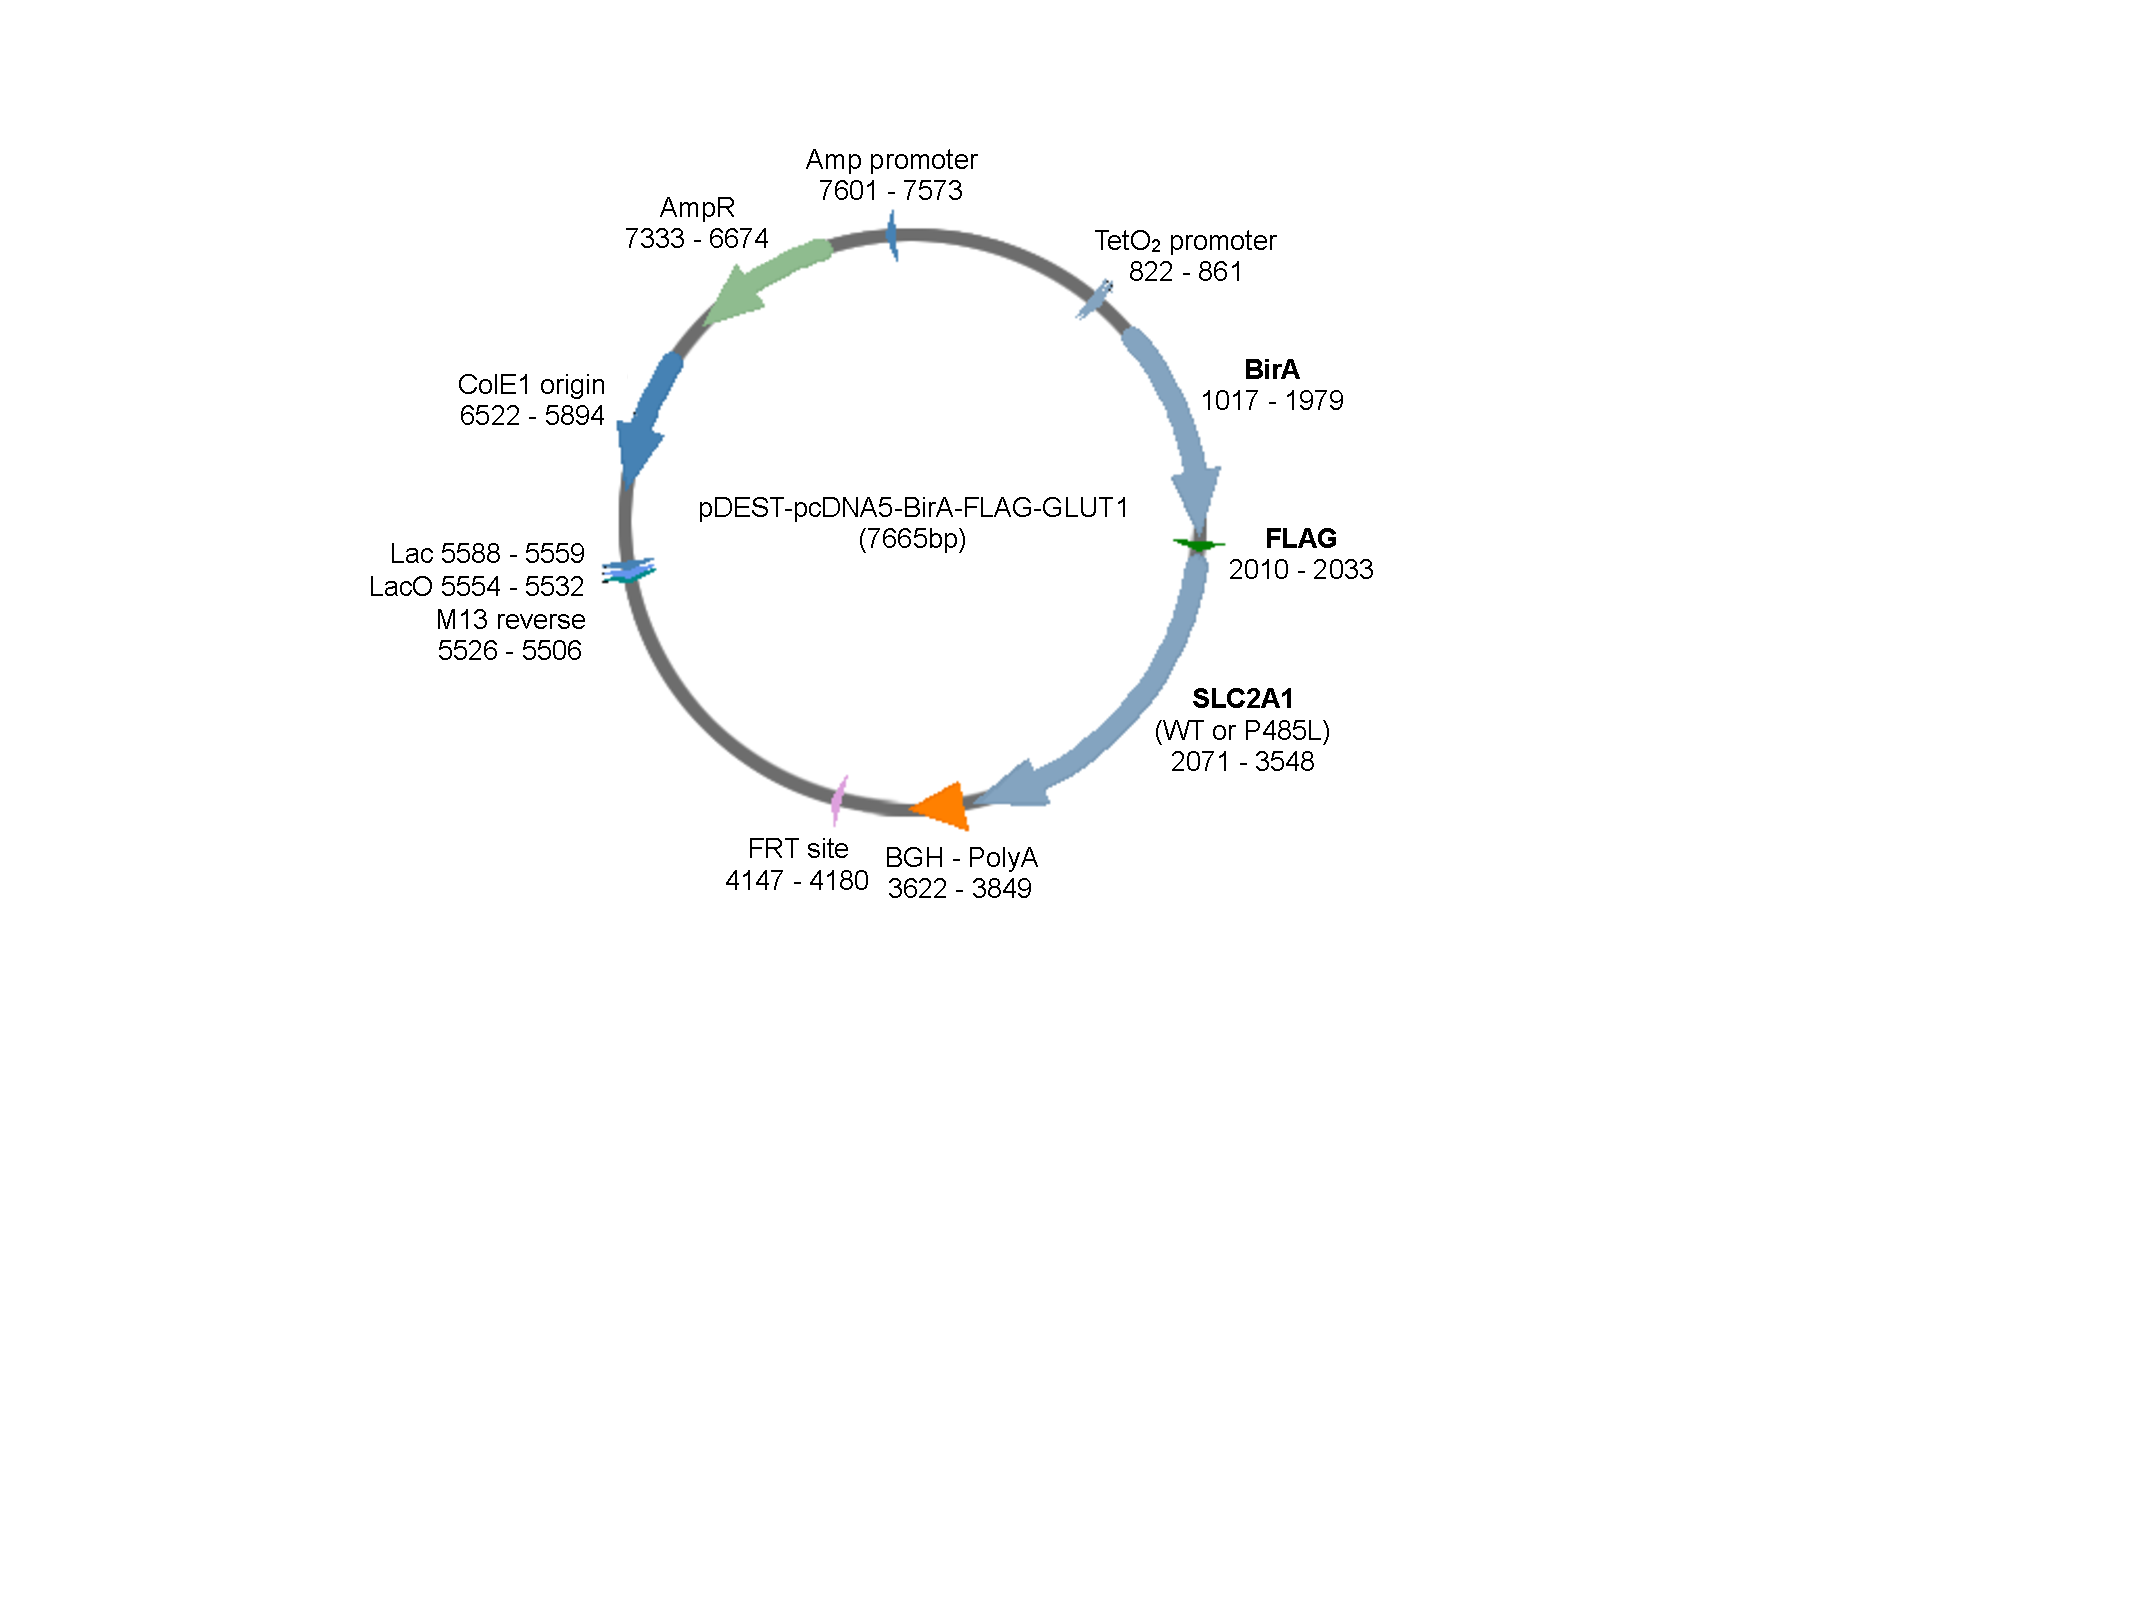
\includegraphics[scale=0.7]{Figures/vector}
\caption{Graphic map of the recombinant plasmid.}
\label{fig:vectors}
\end{figure}
The stable cell lines were stored in cryogenic vials (Croning) in liquid nitrogen. To recover cells, one vial of each cell line was warmed up to \SI{37}{\celsius} and the contents were diluted in 10 mL pre-warmed DMEM (Life Technologies) complemented with 10\% fetal bovine serum (Pan-Biotech). The medium is referred to as complete DMEM in the following. After spinning down at room temperature and 500 rpm for 3 min, the cell pellets were resuspended in 10 mL complete DMEM and seeded in T-75 flasks (CELLSTAR).
\\
\\*
\bfseries{Cell culture}\\
\normalfont Stable HEK293 cells were cultured at \SI{37}{\celsius} and 5\% CO\textsubscript{2} in culture flasks in complete DMEM. Cells were seeded to about 10\% confluency and routinely passaged twice a week as follows: the medium was aspirated and the cells were briefly washed with 4 mL sterile pre-warmed PBS (Life Technologies). To detach the cells 1 mL trypsin-EDTA (0.05\%, Life Technologies) was added and the flask was placed in an incubator at \SI{37}{\celsius} and 5\% CO\textsubscript{2} for 1 min. Trypsin was then inactivated with 9 mL pre-warmed complete DMEM. The medium was gently pipetted to the bottom of the flask in order to recover all the cells and get single-cell suspension. 1 mL of the cell suspension was transferred into 10 mL fresh complete DMEM in a new culture flask which was then placed back in the incubator. The cells would reach approximately 80\% confluency before the next passaging.

\begin{figure}[h]
\centering
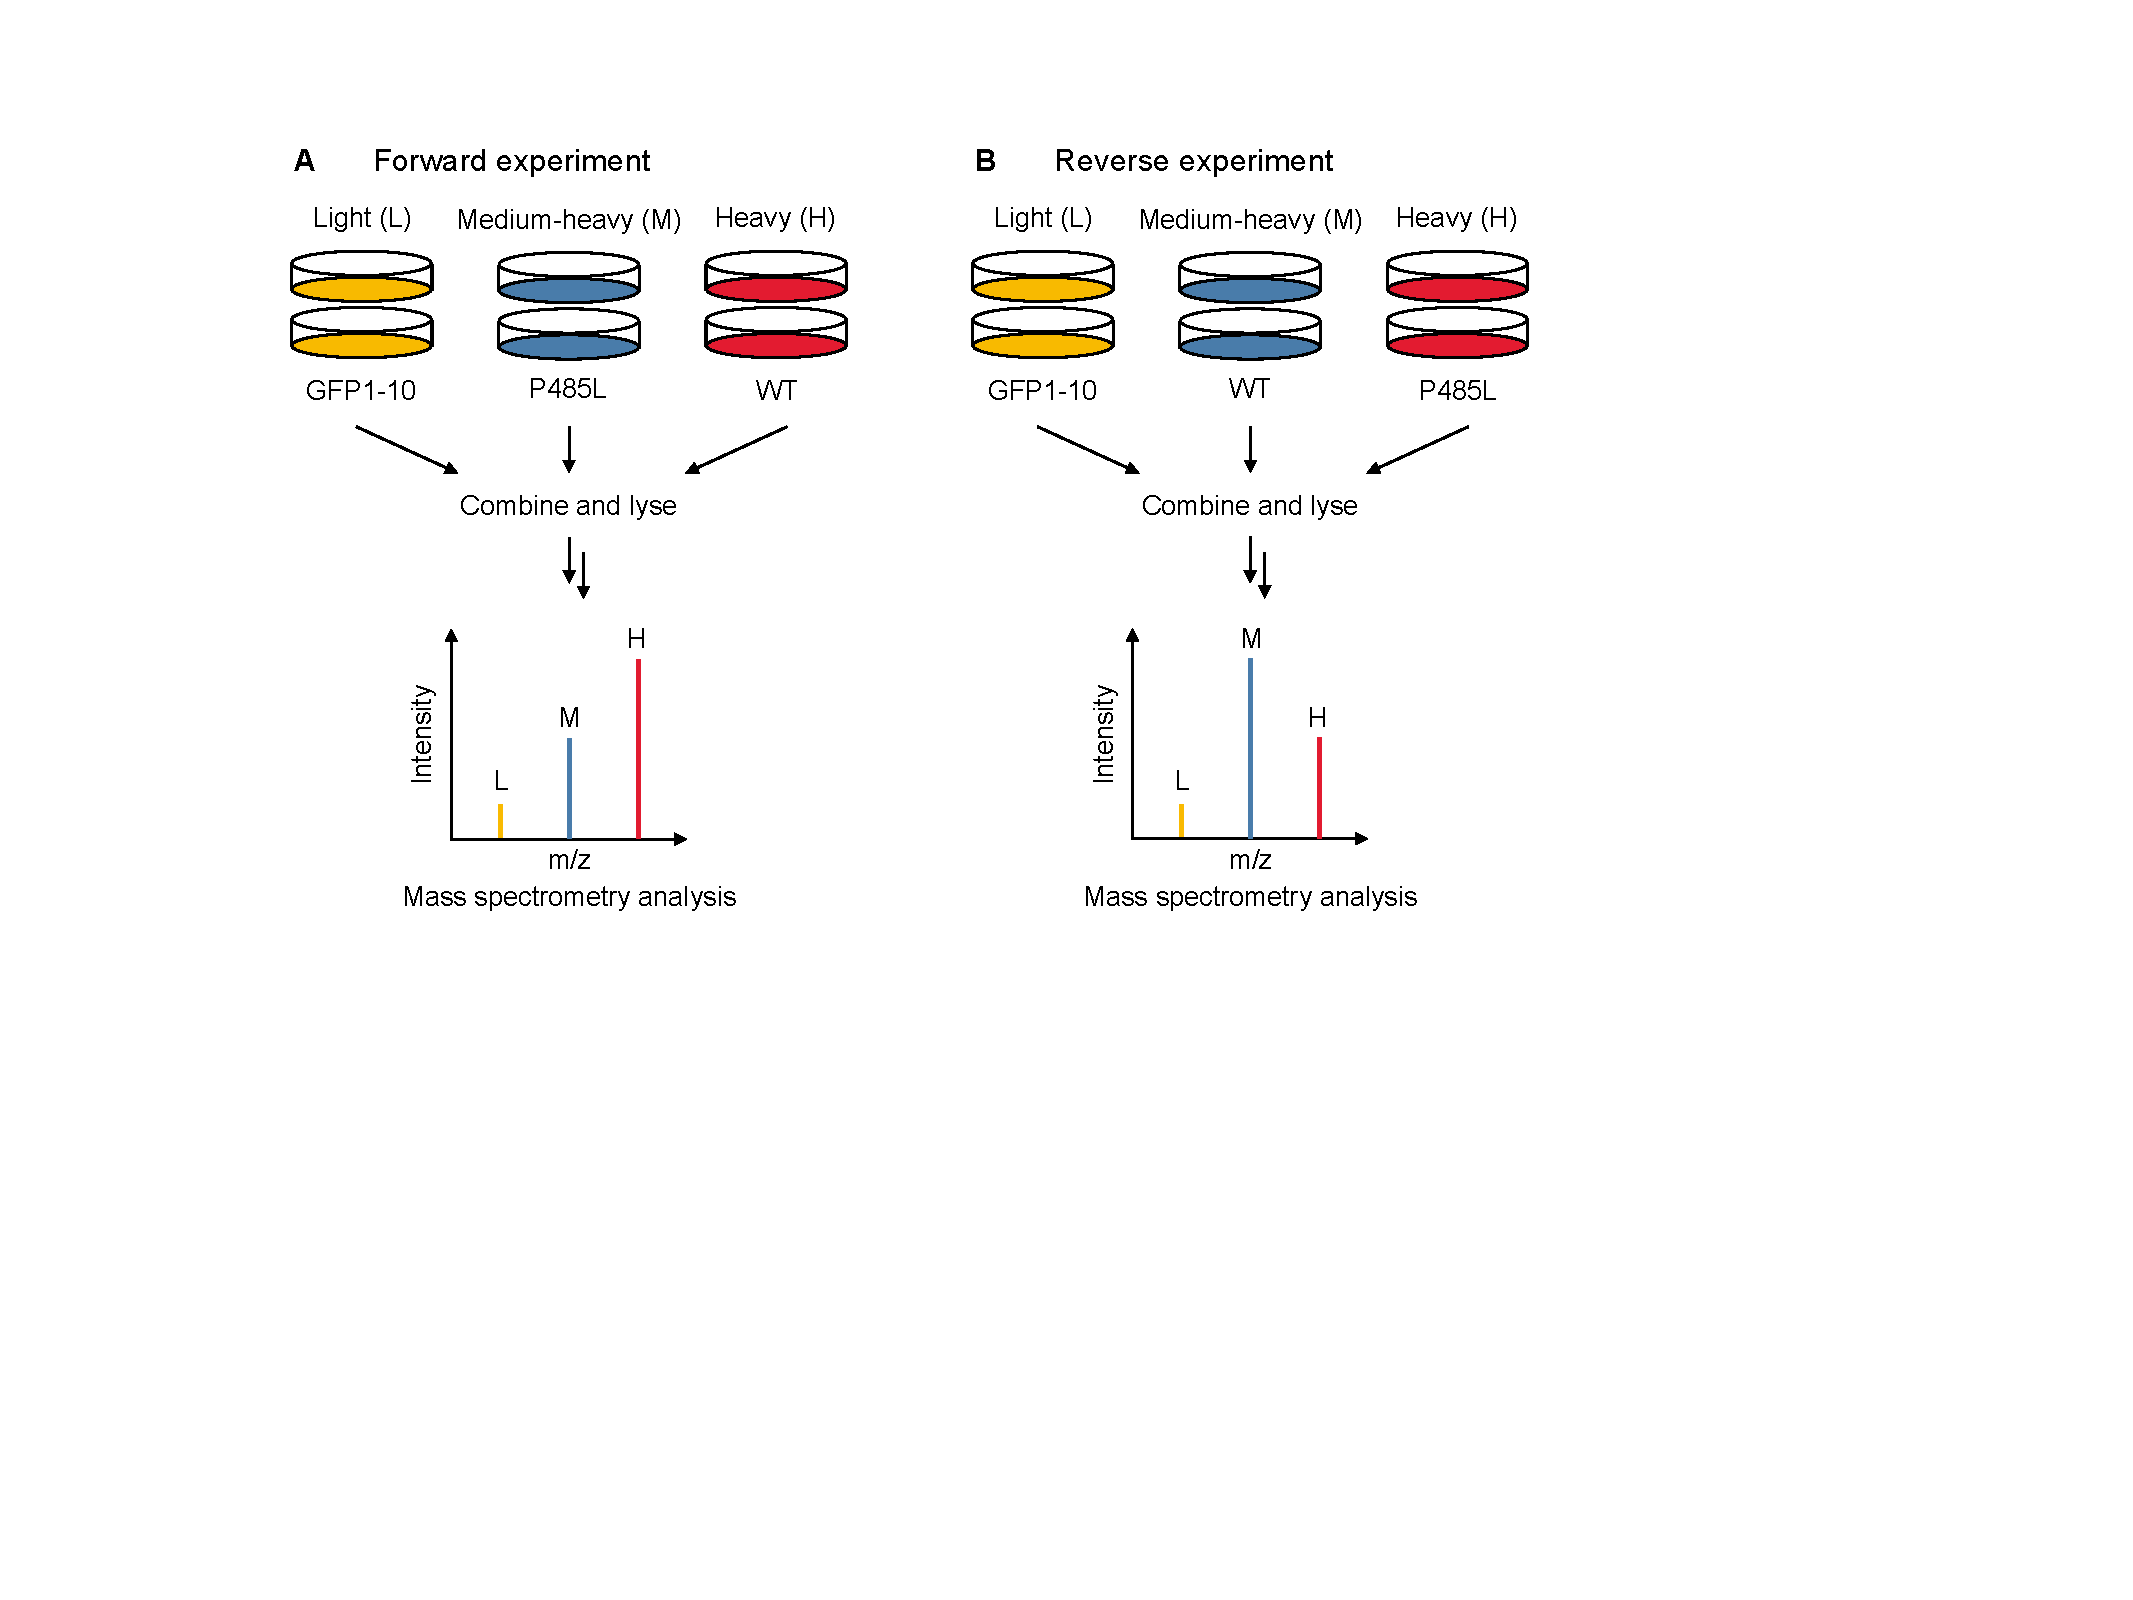
\includegraphics[scale=0.7]{Figures/BioID}
\caption{Experimental setup of triple SILAC labels.}
\label{fig:bioid}
\end{figure}
Cells used for BioID experiments were cultured in SILAC DMEM (Life Technologies) complemented with 2 mM glutamine (Glutamax, Life Technologies), 1 mM pyruvate (Life Technologies), 0.1 mM non-essential amino acids (Life Technologies) and 10\% dialyzed fetal bovine serum (Pan-Biotech). In addition, L-arginine (Arg0, Sigma-Aldrich) and L-lysine (Lys0, Sigma-Aldrich) were added to the Light SILAC DMEM to a final concentration of 0.199 mM and 0.339 mM, respectively. Alternatively, Arg6 and Lys4 or Arg10 and Lys8 were added in place of their Light counterparts to make Medium-heavy SILAC DMEM and Heavy SILAC DMEM, respectively. PBS-EDTA (Lonza) was used to detach the cells when passaging to avoid isotope contamination. After six passages cells were fully labeled as assessed by MS.
% From Koshi: stock conc. are Lys 0.798M, Arg 0.398M (my dilution is 1:2000). DMEM conc: Lys 146mg/L, Arg 84mg/L; if 1:3000 dilution, final conc. should be 1/4 of standard DMEM conc.

For the doxycycline induction experiments unlabeled HEK293 cells were cultured in 6-well plates. The cells were grown to approximately 50\% confluency on the second day after seeding. The medium was removed and 2 mL complete DMEM containing doxycycline (Sigma-Aldrich) was carefully added to each well. After 24 hr or 48 hr the cells were harvested for Western blotting analysis.

For the BioID experiments fully labeled HEK293 cells were seeded in 15 cm plates with approximately 25\% density. Two plates were used for each condition. HEK293 stable cells expressing GFP1-10 were labeled in Light SILAC DMEM and used as negative control cells. Besides the Light control cells, in the forward experiment mutant GLUT1 cells were cultured in Medium-heavy SILAC DMEM and wild-type GLUT1 cells were cultured in Heavy SILAC DMEM (Figure~\ref{fig:bioid} A), while in the reverse label-swap experiment wild-type GLUT1 cells were cultured in Medium-heavy SILAC DMEM and mutant GLUT1 cells were cultured in Heavy SILAC DMEM (Figure~\ref{fig:bioid} B). The cells were grown to 40\%-50\% confluency before being treated with 0.1 {}\textmu g/mL doxycycline and 1 mM biotin (ThermoFisher). After 24 hr, the cells were scraped in ice-cold PBS and collected for further BioID purification and MS analysis.

For the immunofluorescence experiments sterile glass coverslips (Roth, 18 mm diameter, 0.170 mm thickness) were placed in 12-well plates. Poly-L-lysine (0.01\%, Sigma-Aldrich) was added to each well to cover the coverslips. After incubation at room temperature for 5 min, poly-L-lysine was recovered from the wells and stored at \SI{4}{\celsius}. The coverslips were washed twice with sterile H\textsubscript{2}O before being air-dried completely. Unlabeled HEK293 cells were then seeded in the plates with approximately 25\% density. The cells were treated with 0.1 {}\textmu g/mL doxycycline on the second day and subjected to subsequent immunostaining on the third day.
\\
\\*
\bfseries{Western blotting}\\
\normalfont Cells were grown in 6-well plates as described above. After doxycycline or inhibitor treatment, cells were scraped in ice-cold PBS and spun down at 300 rcf, \SI{4}{\celsius} for 4 min. Cell pellets were lyzed for 15 min at room temperature in 100 \textmu L lysis buffer [50 mM ABC solution, 2\% SDS, supplemented with 60 Units/mL benzonase (Sigma-Aldrich) and protease inhibitors (Roche)]. Lysates were spun down at 16 100 rcf for 15 min to remove cell debris and supernatants were transferred to new Eppendorf tubes. For each SDS-PAGE sample, 15 {}\textmu L supernatant was diluted in LDS sample buffer (NOVEX) complemented with 1 {}\textmu L 1M DTT (Sigma-Aldrich) before being heated at \SI{70}{\celsius} for 10 min in a thermoblock. Samples were then loaded onto a 4\%-12\% gel (NOVEX) along with protein ladders (PageRuler Plus, ThermoFisher). Proteins were separated using electrophoresis for 90 min at 150 V in 400 mL MES running buffer (ThermoFisher). 

Before protein transfer a PVDF membrane (Merck Millipore) was activated in methanol for 1 min and equilibrated in ice-cold transfer buffer (25 mM Tris-HCl, 192 mM glycine, 20\% methanol, pH 8.3) for 10 min. Whatman filter papers and sponges were also soaked in transfer buffer for 10 min. A tank blotting system (Invitrogen) was used to transfer the separated proteins to the membrane. In short, a transfer sandwich was prepared with the membrane on the cathode and the gel on the anode. Air bubbles between the gel and membrane were removed by rolling them out with a roller. The cassette was then placed in the transfer tank on ice and the proteins were transferred at a constant current of 250 mA for 2 hr.

After protein transfer the membrane was blocked in 5\% milk powder in TBST (150 mM sodium chloride, 20 mM Tris-HCl, 0.1\% Tween-20, pH 7.6) at room temperature for 30 min. The membrane was then incubated with the primary antibody diluted in blocking buffer while rotating at \SI{4}{\celsius}. The membrane was washed 3 times for 5 min in TBST before being incubated at room temperature for 1 hr with the HRP-conjugated secondary antibody diluted in blocking buffer. The membrane was washed again before the chemiluminescence substrate (PerkinElmer) was applied to the membrane. The chemiluminescent signals were captured using a ChemiDoc MP Imaging System (Bio-Rad) and quantified with Image Lab 5.2.1. The primary and secondary antibodies used in this thesis are summarized in Table~\ref{tab:antibodies}.
\begin{table}[h]
\caption{Antibodies used for Western blotting and their dilutions.}
\label{tab:antibodies}
\small
\centering
\begin{tabular*}{\textwidth}{l@{\extracolsep{\fill}}lll}
\toprule
\tabhead{Antibodies} & \tabhead{Source} & \tabhead{Dilution} & \tabhead{Conjugate}\\
\midrule
Rabbit polyclonal anti-FLAG & Cell Signaling Technology & 1:1000 & HRP\\
Rabbit polyclonal anti-LC3 & Novus Biologicals & 1:1000 & \\
Rat monoclonal anti-HA & Roche & 1:1000 & \\
Mouse monoclonal anti-\textbeta-actin & Sigma-Aldrich & 1:10 000 & \\
Donkey anti-rabbit IgG & GE Healthcare & 1:10 000 & HRP\\
Goat anti-rat IgG & GE Healthcare & 1:15 000 & HRP\\
Sheep anti-mouse IgG & GE Healthcare & 1:25 000 & HRP\\
\bottomrule\\
\end{tabular*}
\end{table}
\\*
\bfseries{Transfection and inhibitor treatments}\\
\begin{figure}[h]
\centering
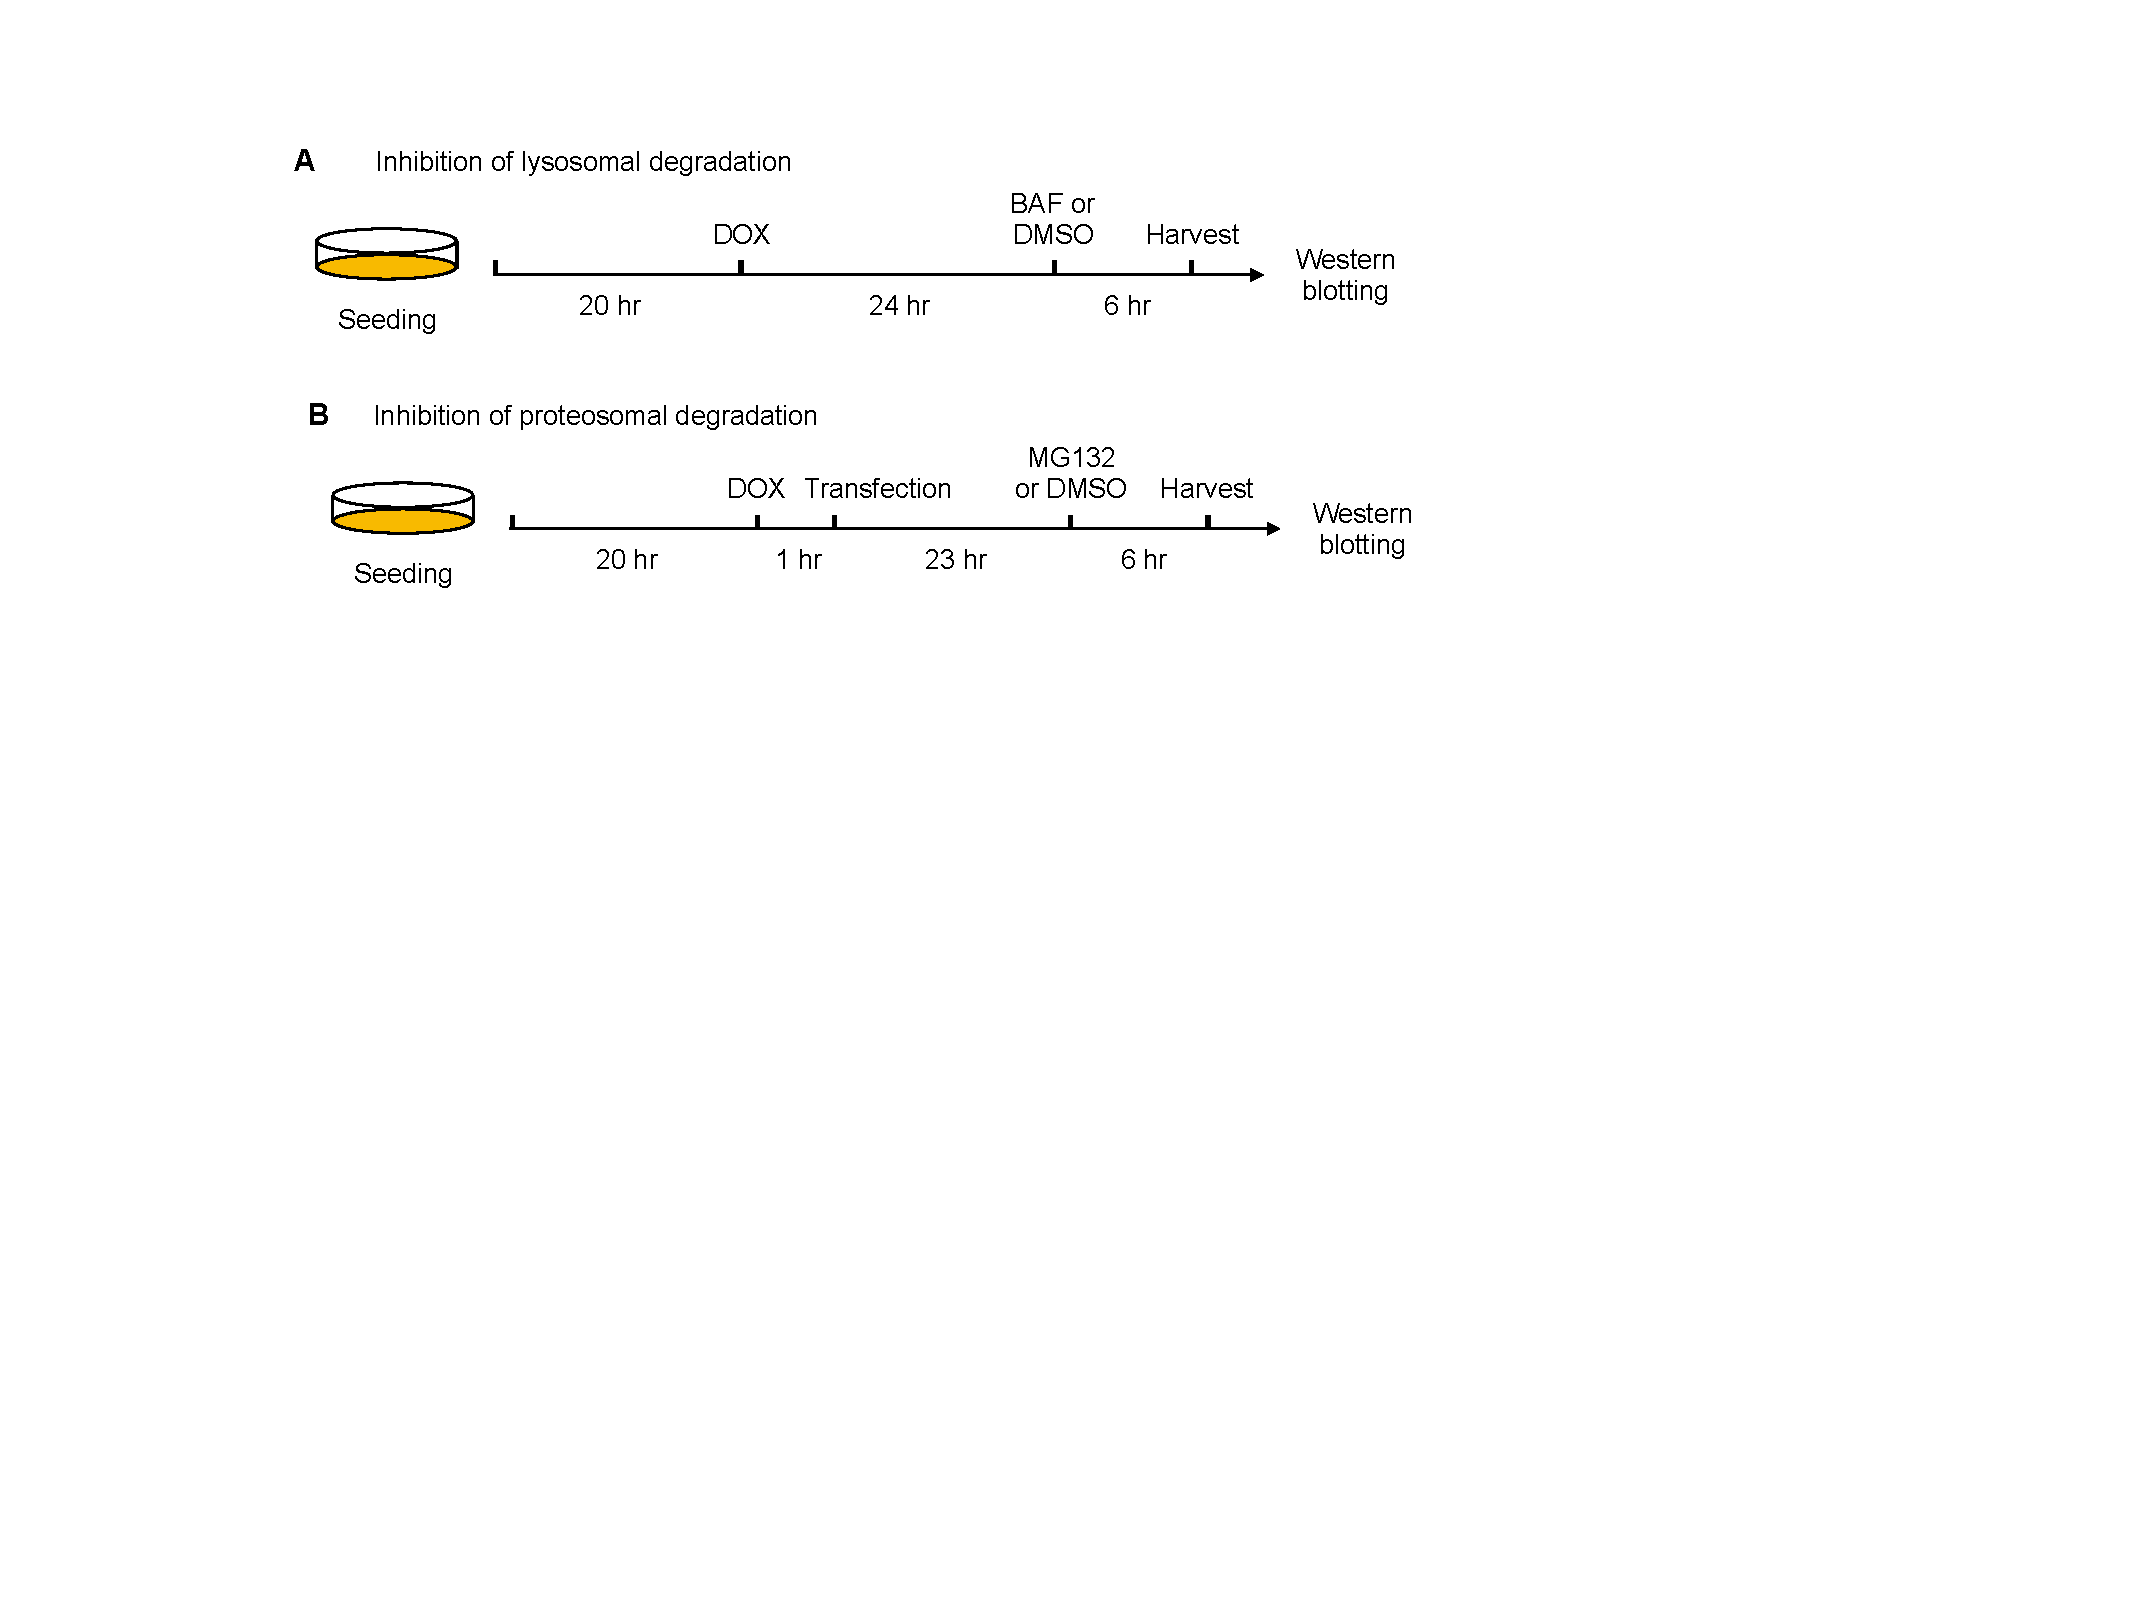
\includegraphics[scale=0.7]{Figures/treatment}
\caption{A timeline of inhibition experiments.}
\label{fig:inhibition}
\end{figure}
\normalfont Inhibitor treatment experiments were performed as the doxycycline (DOX) induction experiments but only with the 24 hr induction time point. In addition to inducing GLUT1 expression with 0.1 \textmu g/mL doxycycline, different inhibitors or DMSO (Biomol) control were added. Lysosomal degradation was inhibited using 250 nM bafilomycin A1 (Invitrogen, BAF) in DMSO for 6 hr before the cells were lysed for Western blotting analysis (Figure~\ref{fig:inhibition} A).

Cells for proteosomal inhibition experiments were transfected with UL21a-HA, an HA-epitope tagged HCMV gene, 1 hr after adding doxycycline. In brief, 20 \textmu g UL21a-HA was mixed with 40 \textmu L jetPRIME (Polyplus) in 2 mL jetPRIME (Polyplus) buffer. After incubation for 10 min, 200 \textmu L of the resulting transfection mix was added drop wise onto the cells in each well. On the next day proteasomes were blocked using 20 mM MG132 (Cayman chemical) in DMSO for 6 hr. The cells were then lysed for Western blotting analysis (Figure~\ref{fig:inhibition} B). The cellular levels of UL21a were taken as the positive control for the inhibitory effect of MG132 treatment.
\\
\\*
\bfseries{BioID and MS analysis}\\
\normalfont Cells scraped from 15 cm plates were spun down at 300 rcf at \SI{4}{\celsius} for 4 min. After resuspension in ice-cold PBS, the triple SILAC labels were combined into a forward and a reverse experiment (Figure~\ref{fig:bioid}). The cells were spun down again and the cell pellets were resuspended in 1.5 mL of RIPA buffer (50 mM tris-HCl, 150 mM NaCl, 1\% NP-40, 1 mM EDTA, 1 mM EGTA, 0.1\% SDS, 1\% sodium deoxycholate, pH 7.5, supplemented with 75 Units/mL benzonase and protease inhibitors). After incubation with agitation at \SI{4}{\celsius} for 1 hr, the lysates were sonicated on ice for 3 min. The lysates were then centrifuged for 20 min at 16 100 rcf at \SI{4}{\celsius} to remove cell debris and the supernatants were transferred to 2 mL Eppendorf tubes.

For affinity purification a 180 {}\textmu L bed volume of streptavidin T1 magnetic beads (Invitrogen) was washed in PBS twice and RIPA buffer once before being resuspended in 200 {}\textmu L RIPA buffer. 100 {}\textmu L of the bead solution was added to each lysate sample. Affinity purification was performed at \SI{4}{\celsius} for 3 hr on a rotating wheel.

The beads were then carefully washed twice in RIPA buffer and twice in TAP lysis buffer (50 mM HEPES-KOH, 100 mM KCl, 10\% glycerol, 2 mM EDTA, 0.1\% NP-40, pH 8.0). The detergents were removed by washing three times in 50 mM ABC. The beads were resuspended in 200 {}\textmu L ABC and 10 {}\textmu L of 10 mM DTT in 50 mM ABC was added to reduce disulfide bonds of proteins. After 30 min incubation in a thermomixer at \SI{30}{\celsius} at 500 rpm, 10 {}\textmu L of 55 mM IAA (Sigma-Aldrich) in 50 mM ABC was added to alkylate the cysteine residues and the samples were incubated in the dark at \SI{30}{\celsius} at 500 rpm for 30 min. The samples then were digested with 1.5 {}\textmu g trypsin (Promega) and incubated overnight at \SI{30}{\celsius} at 1100 rpm. On the next day, the tryptic peptides were separated from beads with a magnetic rack and transferred to fresh 1.5 mL tubes. The digestion was stopped by acidification with 10 \textmu L of 10\% TFA and the tryptic peptides were loaded on C18 StageTip columns for purification~\cite{Rappsilber}. After washing with sample buffer (3\% TFA, 5\% acetonitrile) twice, the peptides were eluted from the columns into an autosampler plate with 50 {}\textmu L buffer B (0,1\% formic acid, 80\% acetonitrile). A vacuum centrifuge (Eppendorf) was used to evaporate the solvent and 10 {}\textmu L buffer A (5\% acetonitrile, 0,1\% formic acid) was added to the samples.

Peptides were separated on a reverse-phase column on a High Performance Liquid Chromatography (HPLC) system (ThermoScientific) with a gradient set up as the following ratios of buffer B in buffer A: 2 min at 250 {}\textmu L/min with a linear gradient from 5\% to 6\% buffer B, 18 min at 200 {}\textmu L/min from 6\% to 8\%, 80 min at 200 {}\textmu L/min from 8\% to 20\%, 80 min at 200 {}\textmu L/min from 20\% to 33\%, 20 min at 200 {}\textmu L/min from 33\% to 45\%, 2 min at 200 {}\textmu L/min from 45\% to 60\%, 1 min at 250 {}\textmu L/min from 60\% to 95\%, 5 min at 250 {}\textmu L/min with 95\% buffer B, 1 min at 250 {}\textmu L/min from 95\% to 75\%, and 5 min at 250 {}\textmu L/min at 75\% buffer B. Peptides were ionized using an electrospray ionization source (ThermoScientific) and analyzed on a Q-Exactive Plus Orbitrap instrument (ThermoScientific). The mass spectrometer was operated with Xcalibur in data-dependent acquisition mode with the following parameters: a full MS scan (resolution: 70 000, scan range: 300 to 1700 m/z, AGC target: 1 000 000 ions, maximum injection time: 120 ms) followed by MS-MS analysis (resolution: 17 500, AGC target: 100 000 ions, maximum injection time: 60 ms) on the top 10 abundant ions.

The resulting raw files were analyzed using MaxQuant 1.5.2.8~\cite{Cox}. The reference human proteome database, consisting of 159 616 entries, was downloaded from the UniProt Knowledgebase on February 28th, 2017. Lys4, Arg6 and Lys8, Arg10 were added to the labels. Variable modifications were set as N-terminal acetylation and oxidation of methionines. The \textit{in silico} digestion of peptides in the reference database was performed with trypsin/P site-specific cleavage. Default global parameters were kept except that "re-quantify" and "match between runs" were turned on. The false discovery rate, assessed by in-parallel searching in a decoy database generated by reversing the reference database, was set to 0.01 at peptide and protein levels. 

The following analysis and graphics were performed using Perseus v1.5.8.4 and R v3.3.3. The resulting 
% cut off
\\
\\*
\bfseries{Transferrin uptake}\\
\normalfont After 24 hr of doxycycline induction, the cells were starved for 1 hr in starvation buffer [serum-free medium supplemented with 20 mM HEPES (Life Technologies)]. Transferrin conjugated with Alexa Fluor 568 (Life Technologies) was diluted in starvation buffer to a final concentration of 10 {}\textmu g/mL and droplets of 35 {}\textmu L transferrin solution were pipetted onto a parafilm in a dark humid chamber. The coverslips were then carefully lifted off the bottom of the plate with forceps and placed face-down on the droplets. The humid chamber was incubated at \SI{37}{\celsius} and 5\% CO\textsubscript{2} for 10 min. After transferrin uptake, the coverslips were washed 3 times for 5 min with PBS supplemented with 10 mM MgCl\textsubscript{2} and 10 mM CaCl\textsubscript{2}, followed by standard immunostaining procedures described as below.
\\
\\*
\bfseries{Immunostaining and confocal microscopy}\\
\normalfont Prior to staining, cell culture medium was aspirated and cells were briefly washed with pre-warmed PBS. The cells were fixed in 4\% PFA for 15 min at room temperature before being washed 3 times for 5 min in PBS. To permeabilize cells and block unspecific binding sites the cells were incubated for 1 hr at room temperature in blocking buffer [5\% goat serum (Sigma-Aldrich), 0.3\% Triton X-100 (Sigma-Aldrich) in PBS]. The primary antibody was diluted in antibody dilution buffer [1\% BSA - Fraction V (Sigma-Aldrich), 0.3\% Triton X-100 in PBS], as indicated in Table~\ref{tab:IF}. The coverslips were placed face-down on droplets of 50 {}\textmu L primary antibody solution on a piece of parafilm in a dark humid chamber. After 1 hr incubation at room temperature, the coverslips were placed face-up in the plate and washed 3 times for 5 min in PBS. Similarly, the coverslips were incubated with secondary antibody solution for 1 hr at room temperature in the humid chamber before being washed for 5 min in PBS. The coverslips were then counterstained with DAPI (0.1 {}\textmu g/mL in PBS, Sigma-Aldrich) for 3 min and washed for 10 min in PBS. Finally, the coverslips were briefly rinsed in Milli-Q H\textsubscript{2}O and mounted with ProLong Gold Antifade Mountant (Life Technologies) on slides. After overnight incubation, the slides were stored at \SI{4}{\celsius} in the dark.

\begin{table}[h]
%\captionsetup{font=normalsize}
\caption{Antibodies for immunofluorescence and their dilutions.}
\label{tab:IF}
\small
\centering
\begin{tabular*}{\textwidth}{l@{\extracolsep{\fill}}lll}
\toprule
\tabhead{Antibodies} & \tabhead{Source} & \tabhead{Dilution} & \tabhead{Conjugate}\\
\midrule
Mouse monoclonal anti-FLAG & Sigma-Aldrich & 1:200 & \\
Rabbit polyclonal anti-GLUT1 & Merck Millipore & 1:500 & \\
Rabbit monoclonal anti-EEA1 & Cell Signaling Technology & 1:100 & \\
Rabbit monoclonal anti-Rab4 & Cell Signaling Technology & 1:100 & \\
Rabbit monoclonal anti-Rab9 & Cell Signaling Technology & 1:100 & \\
Rabbit monoclonal anti-Rab11 & Cell Signaling Technology & 1:100 & \\
Rabbit monoclonal anti-LAMP1 & Cell Signaling Technology & 1:100 & \\
Mouse monoclonal anti-Vti1a & BD Biosciences & 1:100\\
Mouse monoclonal anti-Vti1b & BD Biosciences & 1:100\\
Mouse monoclonal anti-STX6 & BD Biosciences & 1:100\\
Goat anti-mouse IgG (H+L) & Invitrogen & 1:500 & Alexa Fluor 488\\
Goat anti-rabbit IgG (H+L) & Invitrogen & 1:500 & Alexa Fluor 488\\
Donkey anti-rabbit IgG (H+L) & Invitrogen & 1:500 & Alexa Fluor 568\\
Donkey anti-mouse IgG (H+L) & Invitrogen & 1:500 & Alexa Fluor 568\\
\bottomrule
\end{tabular*}
\end{table}
Images in this thesis were acquired using Leica DMI6600 confocal laser scanning microscope with an HCX PL APO 63.0$\times$/1.40 oil objective and Leica Application Suite Advanced Fluorescence (v2.7.3 build 9725) software. As summarized in Table~\ref{tab:laser}, fluorophores were excited using 405 nm laser diode, Argon 488 nm laser (20\% power) or DPSS 561 nm laser and detected using photomultiplier tubes (PMT). The pinhole diameter was set to 95.6 {}\textmu m, scanning mode was unidirectional, line average was 2, sampling speed was 400 Hz. For co-localization studies the zoom was set to 5 and the voxel size was 48.1 nm (width) $\times$ 48.1 nm (height) $\times$ 125.9 nm (depth).

\begin{table}[h]
%\captionsetup{font=normalsize}
\caption{Settings for fluorescence excitation and detection.}
\label{tab:laser}
\small
\centering
\begin{tabular*}{\textwidth}{l@{\extracolsep{\fill}}lllll}
\toprule
\tabhead{Fluorophore} & \tabhead{Laser line} & \tabhead{Laser intensity} & \tabhead{PMT} & \tabhead{PMT gain} & \tabhead{PMT offset}\\
\midrule
DAPI & 405 nm & 8.00\% & 413-477 nm & 619 V & -1\\
Alexa 488 & 488 nm & 12.00\% & 506-598 nm & 646 V & -1\\
Alexa 568 & 561 nm & 15.00\% & 580-710 nm & 619 V & -1\\
\bottomrule
\end{tabular*}
\end{table}
The z-stack confocal microscopy images were further analyzed using ImageJ v1.51j. The stack viewing and color options were set as the default configuration of the Bio-Formats plugin. One z slice was selected in each image to represent all stacks. The brightness and contrast of the channels were uniformly adjusted in each staining experiment and a 10 {}\textmu m scale bar was added to the images.

% colocalization analysis: Imaris.
%----------------------------------------------------------------------------------------

% Define some commands to keep the formatting separated from the content 
 
% Chapter 3

\chapter{Results} % Main chapter title
\label{Chapter3} % For referencing the chapter elsewhere, use \ref{Chapter3} 
\addtocontents{toc}{\setcounter{tocdepth}{1}}
\section{Assessment of inducible GLUT1 expression}
Previous results from the work of our laboratory showed that the GLUT1\textsuperscript{P485L} mutation leads to specific interaction with clathrin and the internalization of the protein. In order to further investigate the role and functional effects of the mutation, we used two Flp-In T-Rex HEK293 cell lines containing inducible BirA-FLAG epitope-tagged full length wild-type or mutant GLUT1 (Figure~\ref{fig:vectors}). The cells constitutively express Tet repressor (TetR) which binds to the TetO\textsubscript{2} sequence in the promoter of transgenic GLUT1~\cite{Hillen}. Upon addition, tetracycline binds to the TetR, causing the release of TetR from TetO\textsubscript{2} and induction of transgene transcription~\cite{Hillen}. In this thesis doxycycline was used as a relatively stable tetracycline derivative to induce the expression of the BirA-FLAG tagged GLUT1 variants~\cite{Xu}.

To determine the optimal conditions for inducible expression, GLUT1 wild-type and mutant cells were grown in different concentrations of doxycycline for 24 hr and the expression of the GLUT1 protein was analyzed by Western blotting with an anti-FLAG antibody. No expression of FLAG-tagged GLUT1 was detected in the absence of doxycycline (Figure~\ref{fig:wb} A). Compared with 0.1 \textmu g/mL doxycycline, induction with 1 \textmu g/mL doxycycline resulted in higher GLUT1 levels in wild-type cells, whereas in mutant cells the GLUT1 expression was not significantly altered (Figure~\ref{fig:wb} A and C). The results showed that the lower dose of doxycycline was sufficient for induction of the system. 

Additionally, GLUT1 protein expression was quantified after 24 hr and 48 hr of doxycycline induction. Further increase in the induction time did not result in increased GLUT1 levels in wild-type cells, but actually decreased the expression in mutant cells compared to the 24 hr time point (Figure~\ref{fig:wb} B and D). Therefore the induction with 0.1 \textmu g/mL doxycycline for 24 hr was selected in the following experiments to reduce toxic side effects of the drug~\cite{Zeltser}.

\begin{figure}[h]
\centering
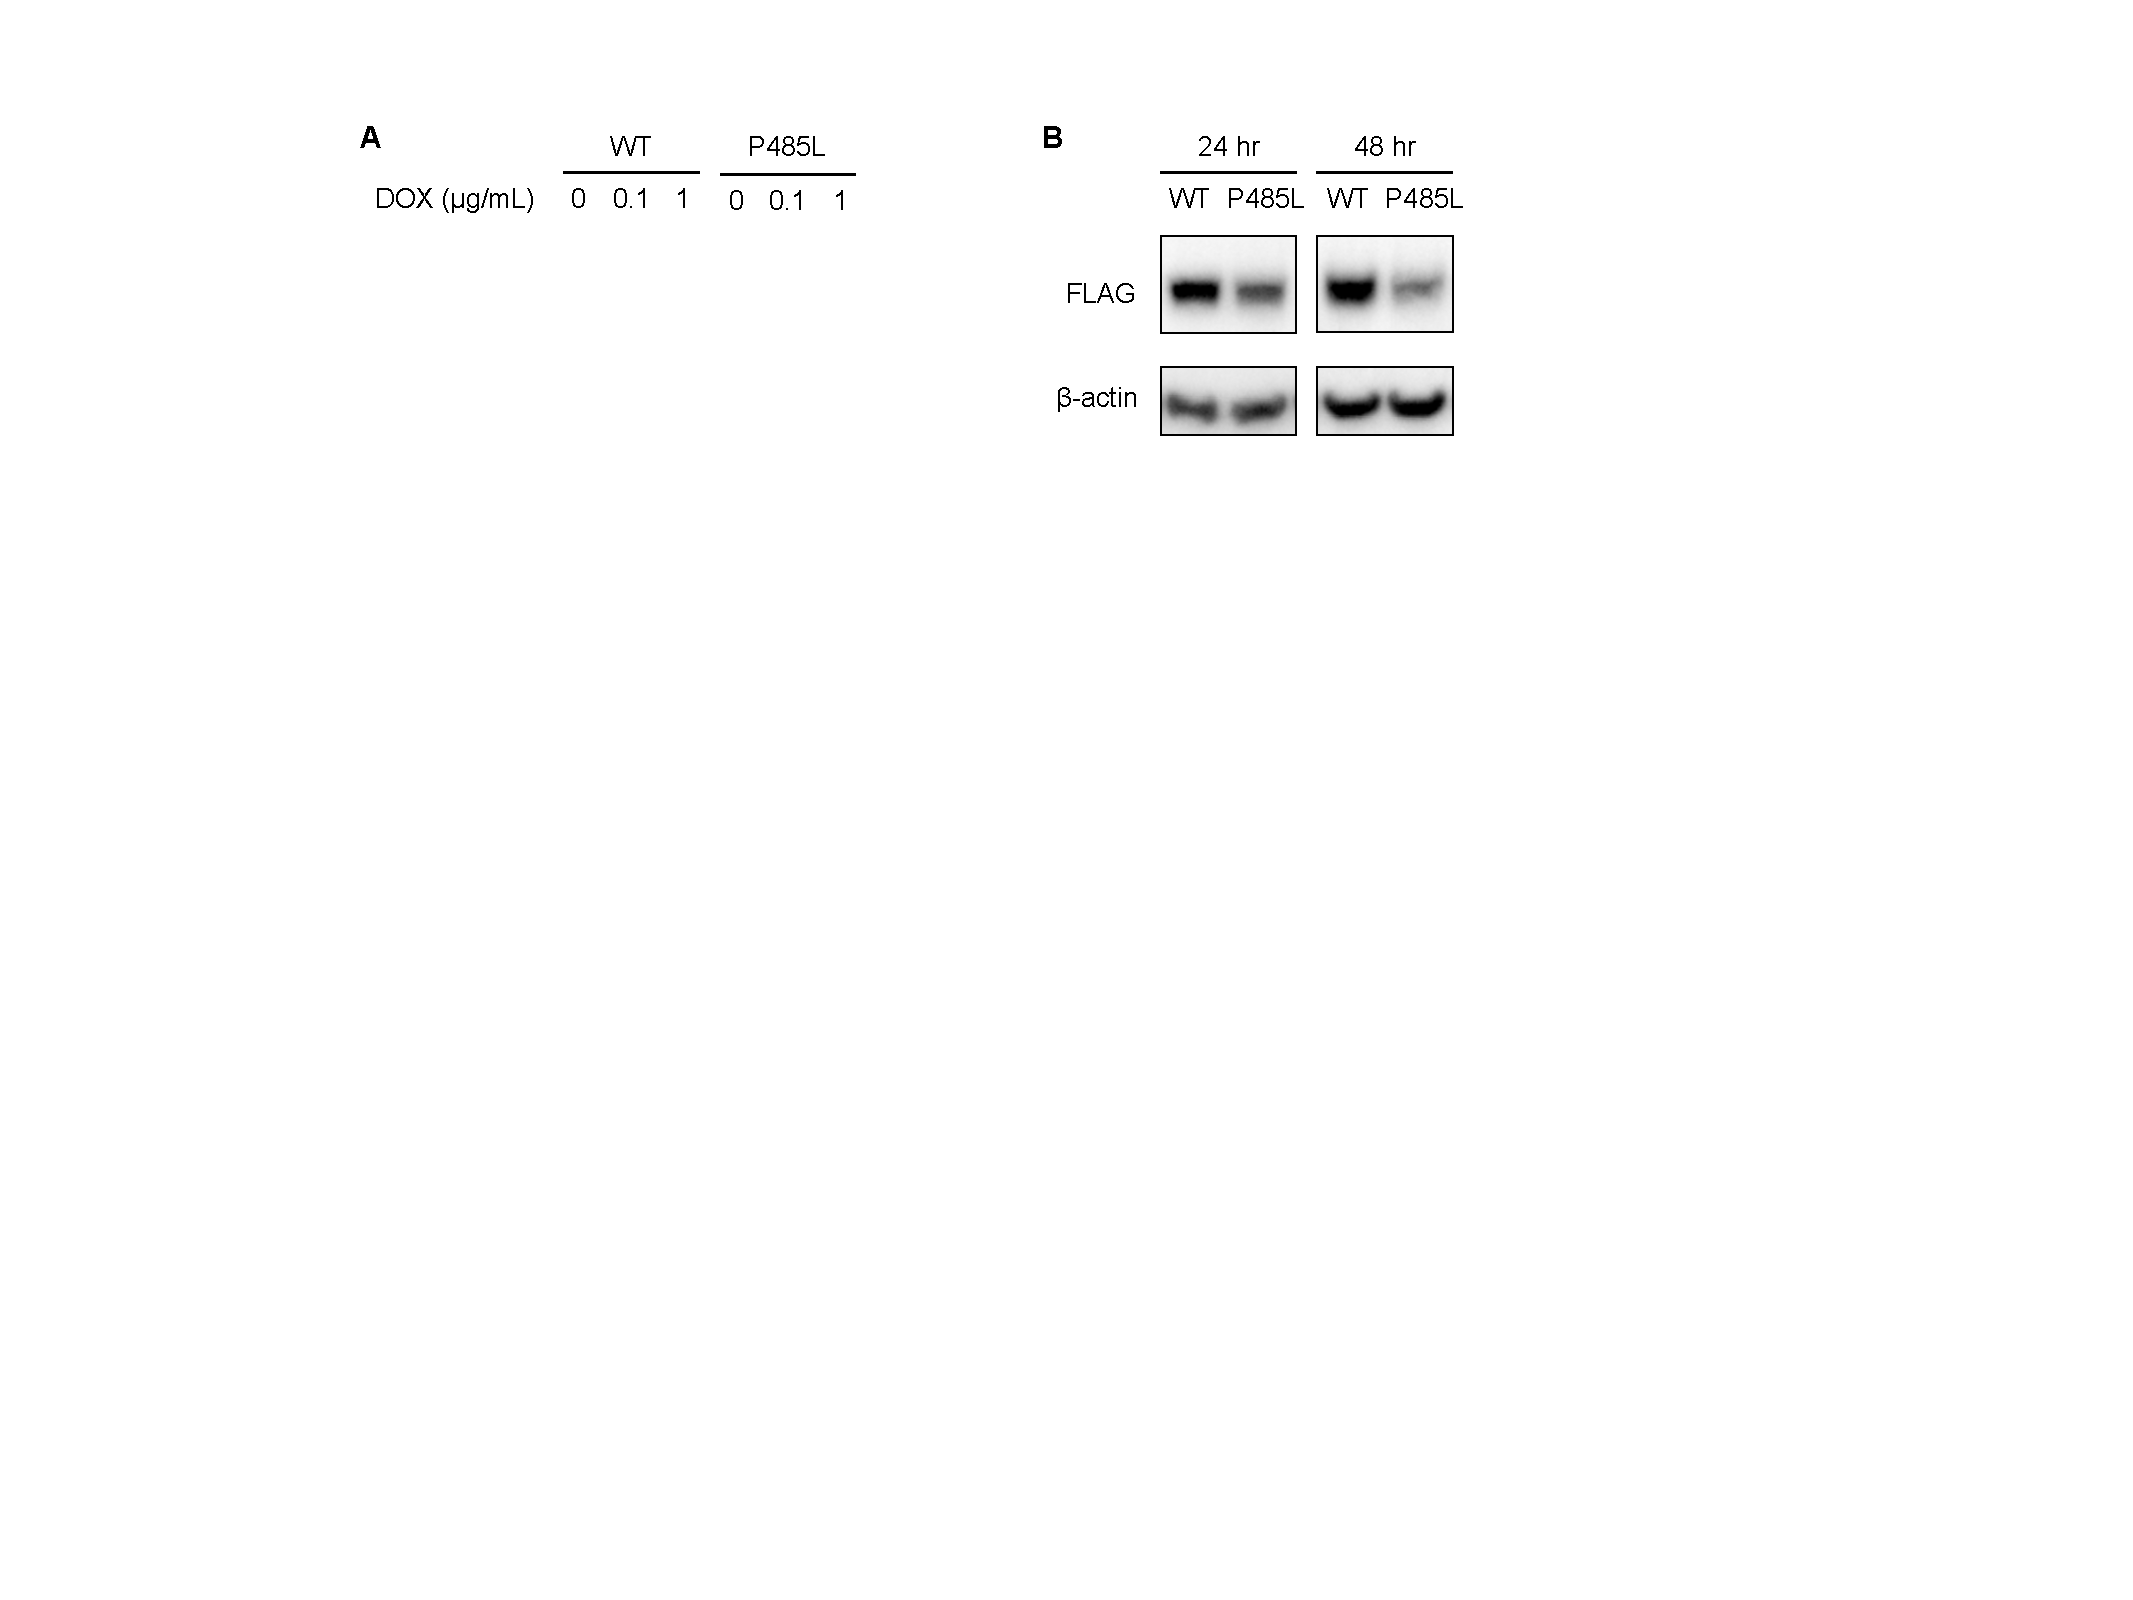
\includegraphics[scale=0.7]{Figures/WB}
\caption{The doxycycline-inducible expression of GLUT1 variants.}
%\smallskip
\vspace*{-3mm}
\small \justify
Different conditions were investigated to induce the expression of BirA-FLAG tagged GLUT1 with doxycycline. GLUT1 wild-type (WT) and mutant (P485L) cells were treated with varying concentrations of doxycycline (0, 0.1 or 1 \textmu g/mL) for 24 hr and analyzed with Western blotting (A). The inducible expression of GLUT1 was also compared between 24 hr and 48 hr induction with 0.1 \textmu g/mL doxycycline (B). Quantification of GLUT1 levels was achieved by normalizing to \textbeta -actin (C, D).
\label{fig:wb}
\end{figure}
Furthermore, the doxycycline-inducible expression of GLUT1 was confirmed by immunofluorescence confocal microscopy. A different anti-FLAG antibody (see "Methods" section) was used to analyze transgene expression with or without doxycycline treatment in both cell lines. Interestingly, although leakiness in expression was not detected in Western blotting, a small subpopulation of uninduced wild-type and mutant cells showed transgene expression in immunofluorescence microscopy (Figure~\ref{fig:if} A and B), 
% In addition, a low basal expression of FLAG-tagged GLUT1 was visible under stronger laser excitation in uninduced wild-type cells, Supplementary fig???, 
suggesting the existence of leaky expression from the Tet promoter in the absence of doxycycline~\cite{Pham,Senkel}. 
In consistence with Western blotting results, strong and roughly uniform expression in response to doxycycline was observed in wild-type and mutant cells (Figure~\ref{fig:if} C and D). 
\begin{figure}[h]
\centering
\includegraphics[scale=0.7]{Figures/if}
\caption{The inducible expression of GLUT1 variants assessed by immunofluorescence microscopy.}
\vspace*{-3mm}
\small \justify
GLUT1 wild-type (WT) and mutant (P485L) cells were cultured on coverslips for 24 hr either in the absence (A, B) or presence (C, D) of 0.1 {}\textmu g/mL doxycycline. Immunostaining of BirA-FLAG tagged GLUT1 was performed with monoclonal mouse anti-FLAG and Alexa 488-conjugated anti-mouse antibodies (green). Cell nuclei were identified by DAPI staining (blue). Scale = 10 \textmu m.
\label{fig:if}
\end{figure}
%As expected, ARF localized to nucleolar regions (the compact circular regions of higher intensity as pointed by the arrow in panel A) while HA-RBP1 demonstrated strong nuclear localization with nucleolar exclusion, as shown by the dark nucleolar regions in panel B. Panel C confirms that RBP2 is localized exclusively to the nucleus. Panel D illustrates that the rabbit polyclonal ?-RBP2 antibody cannot be used in immunofluorescence because of the high amount of non-specific background signal it produces. Trials were done at various dilutions but all were negative and produced the same non-specific noise (data not shown). 

\section{Effect of blocking proteolysis on GLUT1 levels}
Despite the approximately uniform expression within both cell lines, a lower expression level of the FLAG-tagged GLUT1 was observed in mutant cells than in wild-type cells (Figure~\ref{fig:wb}). We thus speculated that the mutant protein might undergo degradation through proteolytic pathways. A rescue experiment was designed to determine the effect of proteolysis on GLUT1 levels by using proteolytic inhibitors Bafilomycin A1 or MG132 to block lysosomal degradation or proteosomal degradation, respectively~\cite{Tanida,Lee.2}. The GLUT1 levels in cells with or without inhibitor treatment were quantified by Western blotting analyses.
%(Figure~\ref{fig:wb2}). 

Bafilomycin A1 inhibits the vacuolar type H\textsuperscript{+}-ATPase complex necessary for lysosomal acidification, thus blocks protein degradation in lysosomes~\cite{Yamamoto,Klionsky}. The inhibitory effect of Bafilomycin A1 was confirmed by the accumulation of LC3-phosphatidylethanolamine conjugate (LC3-II) upon inhibitor treatment (Figure~\ref{fig:wb2} A). Surprisingly, the inhibition decreased wild-type GLUT1 levels by approximately 10\% in comparison to the untreated control group, whereas in mutant cells the inhibition increased GLUT1 levels by around 30\% (Figure~\ref{fig:wb2} B). These results suggest that lysosomal degradation might be partially responsible for the differential GLUT1 protein levels in the two cell lines, but independent sets of experiments and quantification need to be repeated.

\begin{figure}[h]
\centering
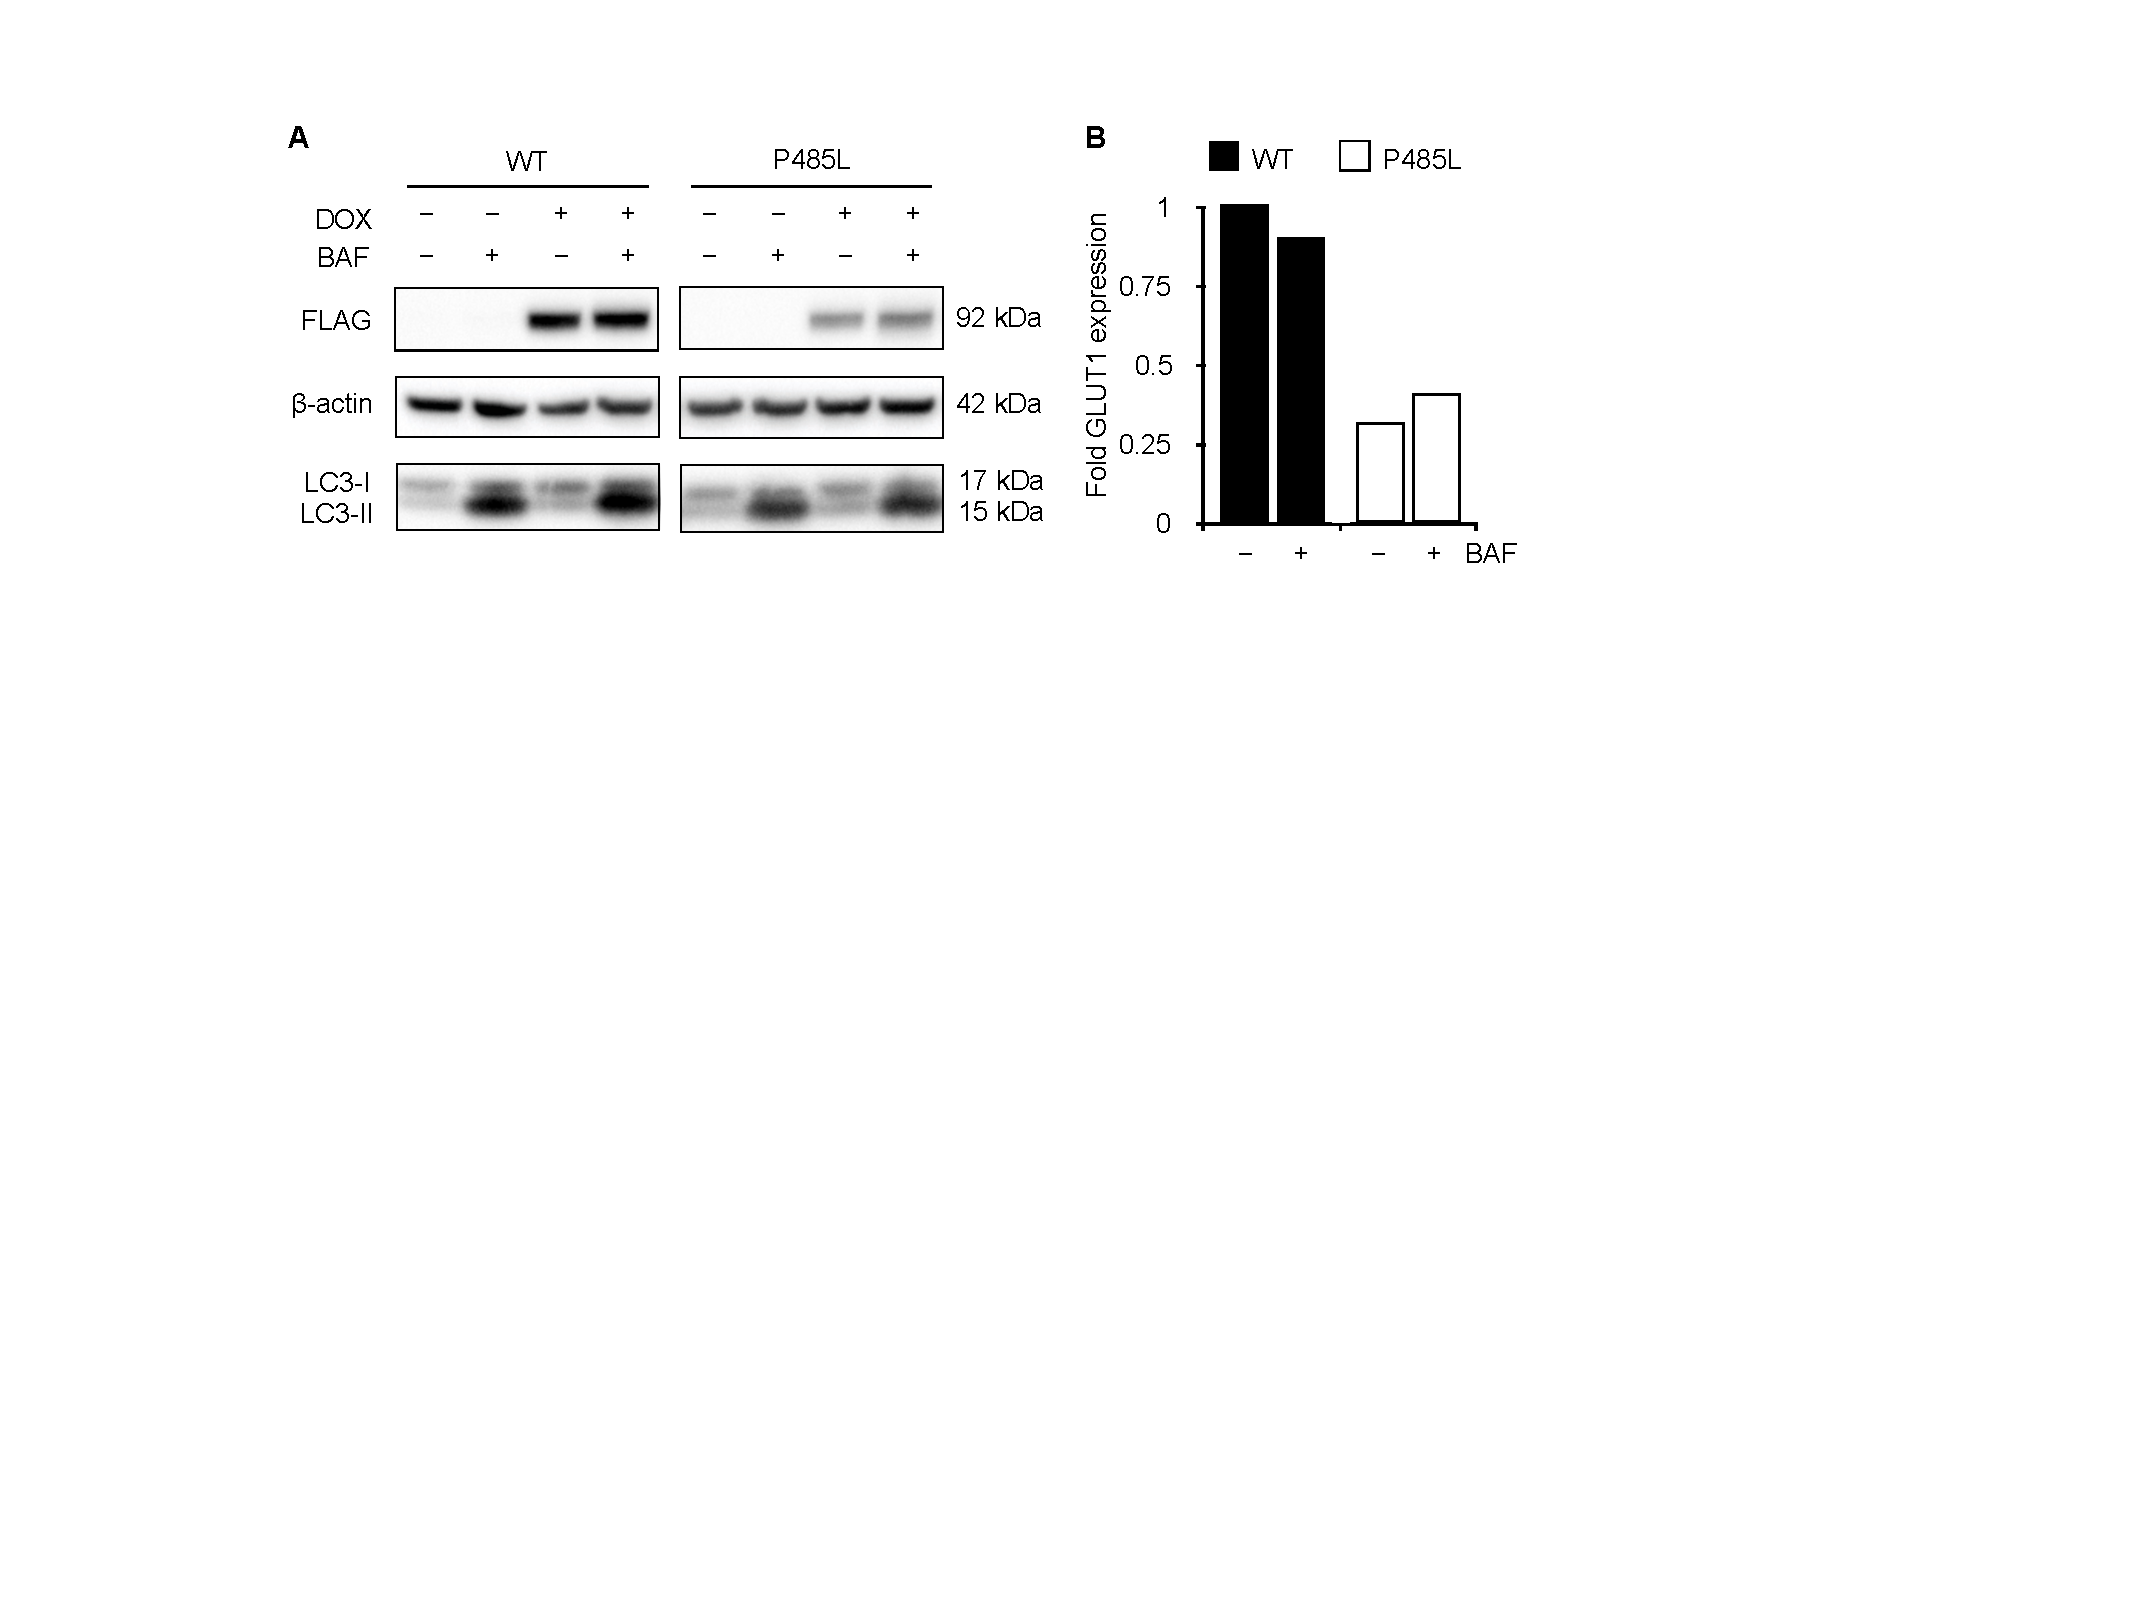
\includegraphics[scale=0.7]{Figures/wb2}
\caption{The effect of blocking lysosomal degradation on GLUT1 levels.}
\vspace*{-3mm}
\small \justify
GLUT1 wild-type (WT) and mutant (P485L) cells were incubated in 0.1 \textmu g/mL doxycycline for 18 hr before Bafilomycin A1 (BAF, final concentration: 250 nM) or carrier control (DMSO) was added. After 6 hr of drug treatment, the cells were lysed and the GLUT1 levels were analyzed in Western blotting (A). Quantification of GLUT1 levels in induced cells was achieved by normalizing to \textbeta -actin (B).
\label{fig:wb2}
\end{figure}
To demonstrate that the proteosomal inhibitor MG132 did decrease proteosomal degradation, cells were transfected with HA epitope-tagged UL21a after doxycycline induction. UL21a has been reported to encode the viral protein pUL21a, a short-lived cytoplasmic protein targeted for proteosome-dependent degradation and can be drastically stabilized in the presence of MG132~\cite{Fehr}. The cells were treated with MG132 or DMSO control after UL21a transfection, and analyzed for the accumulation of HA-tagged pUL21a and FLAG-tagged GLUT1 levels by Western blotting. The accumulation of pUL21a was observed after MG132 treatment, but no significant effect of proteosomal inhibition was shown on wild-type and mutant GLUT1 levels (Figure~\ref{fig:wb3}).

\begin{figure}[h]
\centering
\includegraphics[scale=0.7]{Figures/wb3}
\caption{The effect of blocking proteosomal degradation on GLUT1 levels.}
\vspace*{-3mm}
\small \justify
GLUT1 wild-type (WT) and mutant (P485L) cells were incubated in 0.1 \textmu g/mL doxycycline for 1 hr before being transfected with HA-UL21a. At 17 hr after transfection, MG132 (final concentration: 20 mM) or DMSO control. Cells lysates were collected 6 hr later and analyzed by immunoblotting with an anti-FLAG antibody to determine GLUT1 levels and an anti-HA antibody for pUL21a levels (A). The GLUT1 level in doxycycline induced cells were quantified by normalizing to \textbeta -actin (B).
\label{fig:wb3}
\end{figure}
%we examined LC3-II or p62 levels in serum-starved cellseither in the absence, or presence of bafilomycin A1, an agent thatinhibits lysosomal acidification and/or inhibits autophagosome-lysosome fusion; this treatment leads to reduced degradation andhence, accumulation of autophagy substrates A Role for Presenilins in Autophagy Revisited: Normal Acidification of Lysosomes in Cells Lacking PSEN1 and PSEN2 (PDF Download Available). Available from: https://www.researchgate.net/publication/227858130_A_Role_for_Presenilins_in_Autophagy_Revisited_Normal_Acidification_of_Lysosomes_in_Cells_Lacking_PSEN1_and_PSEN2 [accessed Jul 13, 2017].
%LC3-II levels were elevated in cultured WT-ES cells(Fig. 1A, compare lanes 1, 2)
\section{Cellular localization of GLUT1 variants}
The plasma membrane localization of wild-type GLUT1 has been well demonstrated in sequence and structure-based studies~\cite{Mueckler.2,Hresko,Hruz}.
To compare the localization of wild-type and mutant GLUT1, we examined the localization in the two stable cell lines by immunofluorescent microscopy. Expression of the FLAG-tagged wild-type GLUT1 was clearly detected on the cell surface (Figure~\ref{fig:glut1} B). Conversely, the FLAG-tagged mutant GLUT1 was mostly localized in intracellular regions (Figure~\ref{fig:glut1} D). Additionally, this differential localization was confirmed by using an anti-GLUT1 antibody (Figure~\ref{fig:glut1} A and C).

\begin{figure}[h]
\centering
\includegraphics[scale=0.7]{Figures/glut1}
\caption{The differential cellular localization of GLUT1 variants.}
\vspace*{-3mm}
\small \justify
Localization of GLUT1 wild-type (WT) and mutant (P485L) was analyzed in HEK293 cells induced with 0.1 \textmu g/mL doxycycline for 24 hr. Immunostaining of the FLAG-tagged GLUT1 variants was performed with rabbit anti-GLUT1 and Alexa 488-conjugated anti-rabbit antibodies (green, A and D), as well as mouse anti-FLAG and Alexa 568-conjugated anti-mouse antibodies (red, B and E). The overlay images with DAPI-stained nuclei were also shown (C and F). Scale = 10 \textmu m.
\label{fig:glut1}
\end{figure}
\section{Proximity labeling of GLUT1 variants}
In order to systematically characterize the subcellular localization of the wild-type and mutant GLUT1, proximity-dependent biotinylation (BioID) was used to label neighboring proteins within approximately 20 nm of the BirA-tagged GLUT1 variants~\cite{Kim,Dong}. The BirA enzyme is fused to the N-terminal end of FLAG-GLUT1 and positioned on the cytoplasmic face of the plasma membrane (see "Introduction", Figure~\ref{fig:topo}). Three-state stable isotope labeling with amino acids in cell culture (SILAC) in combination with mass spectrometry analysis was used to quantitatively identify the \textit{in situ} biotinylated proteins. A HEK293 stable cell line containing the GFP1-10 transgene was used as nonbiotinylated negative control in the light channel (See "Methods", Figure~\ref{fig:bioid}). 

Consistent with microscopy results shown in Figure~\ref{fig:glut1}, many of the specific proximal proteins of the wild-type GLUT1 are either transmembrane proteins on the cell surface, such as members of the SLC superfamily (SLC4A7, SLC1A5 etc), or cytosolic proteins that peripherally associate with transmembrane proteins, such as ephrin ligands (EFNB1, EFNB2) (Figure~\ref{fig:bioid2})~\cite{He,Himanen}. 
\begin{figure}[h]
\centering
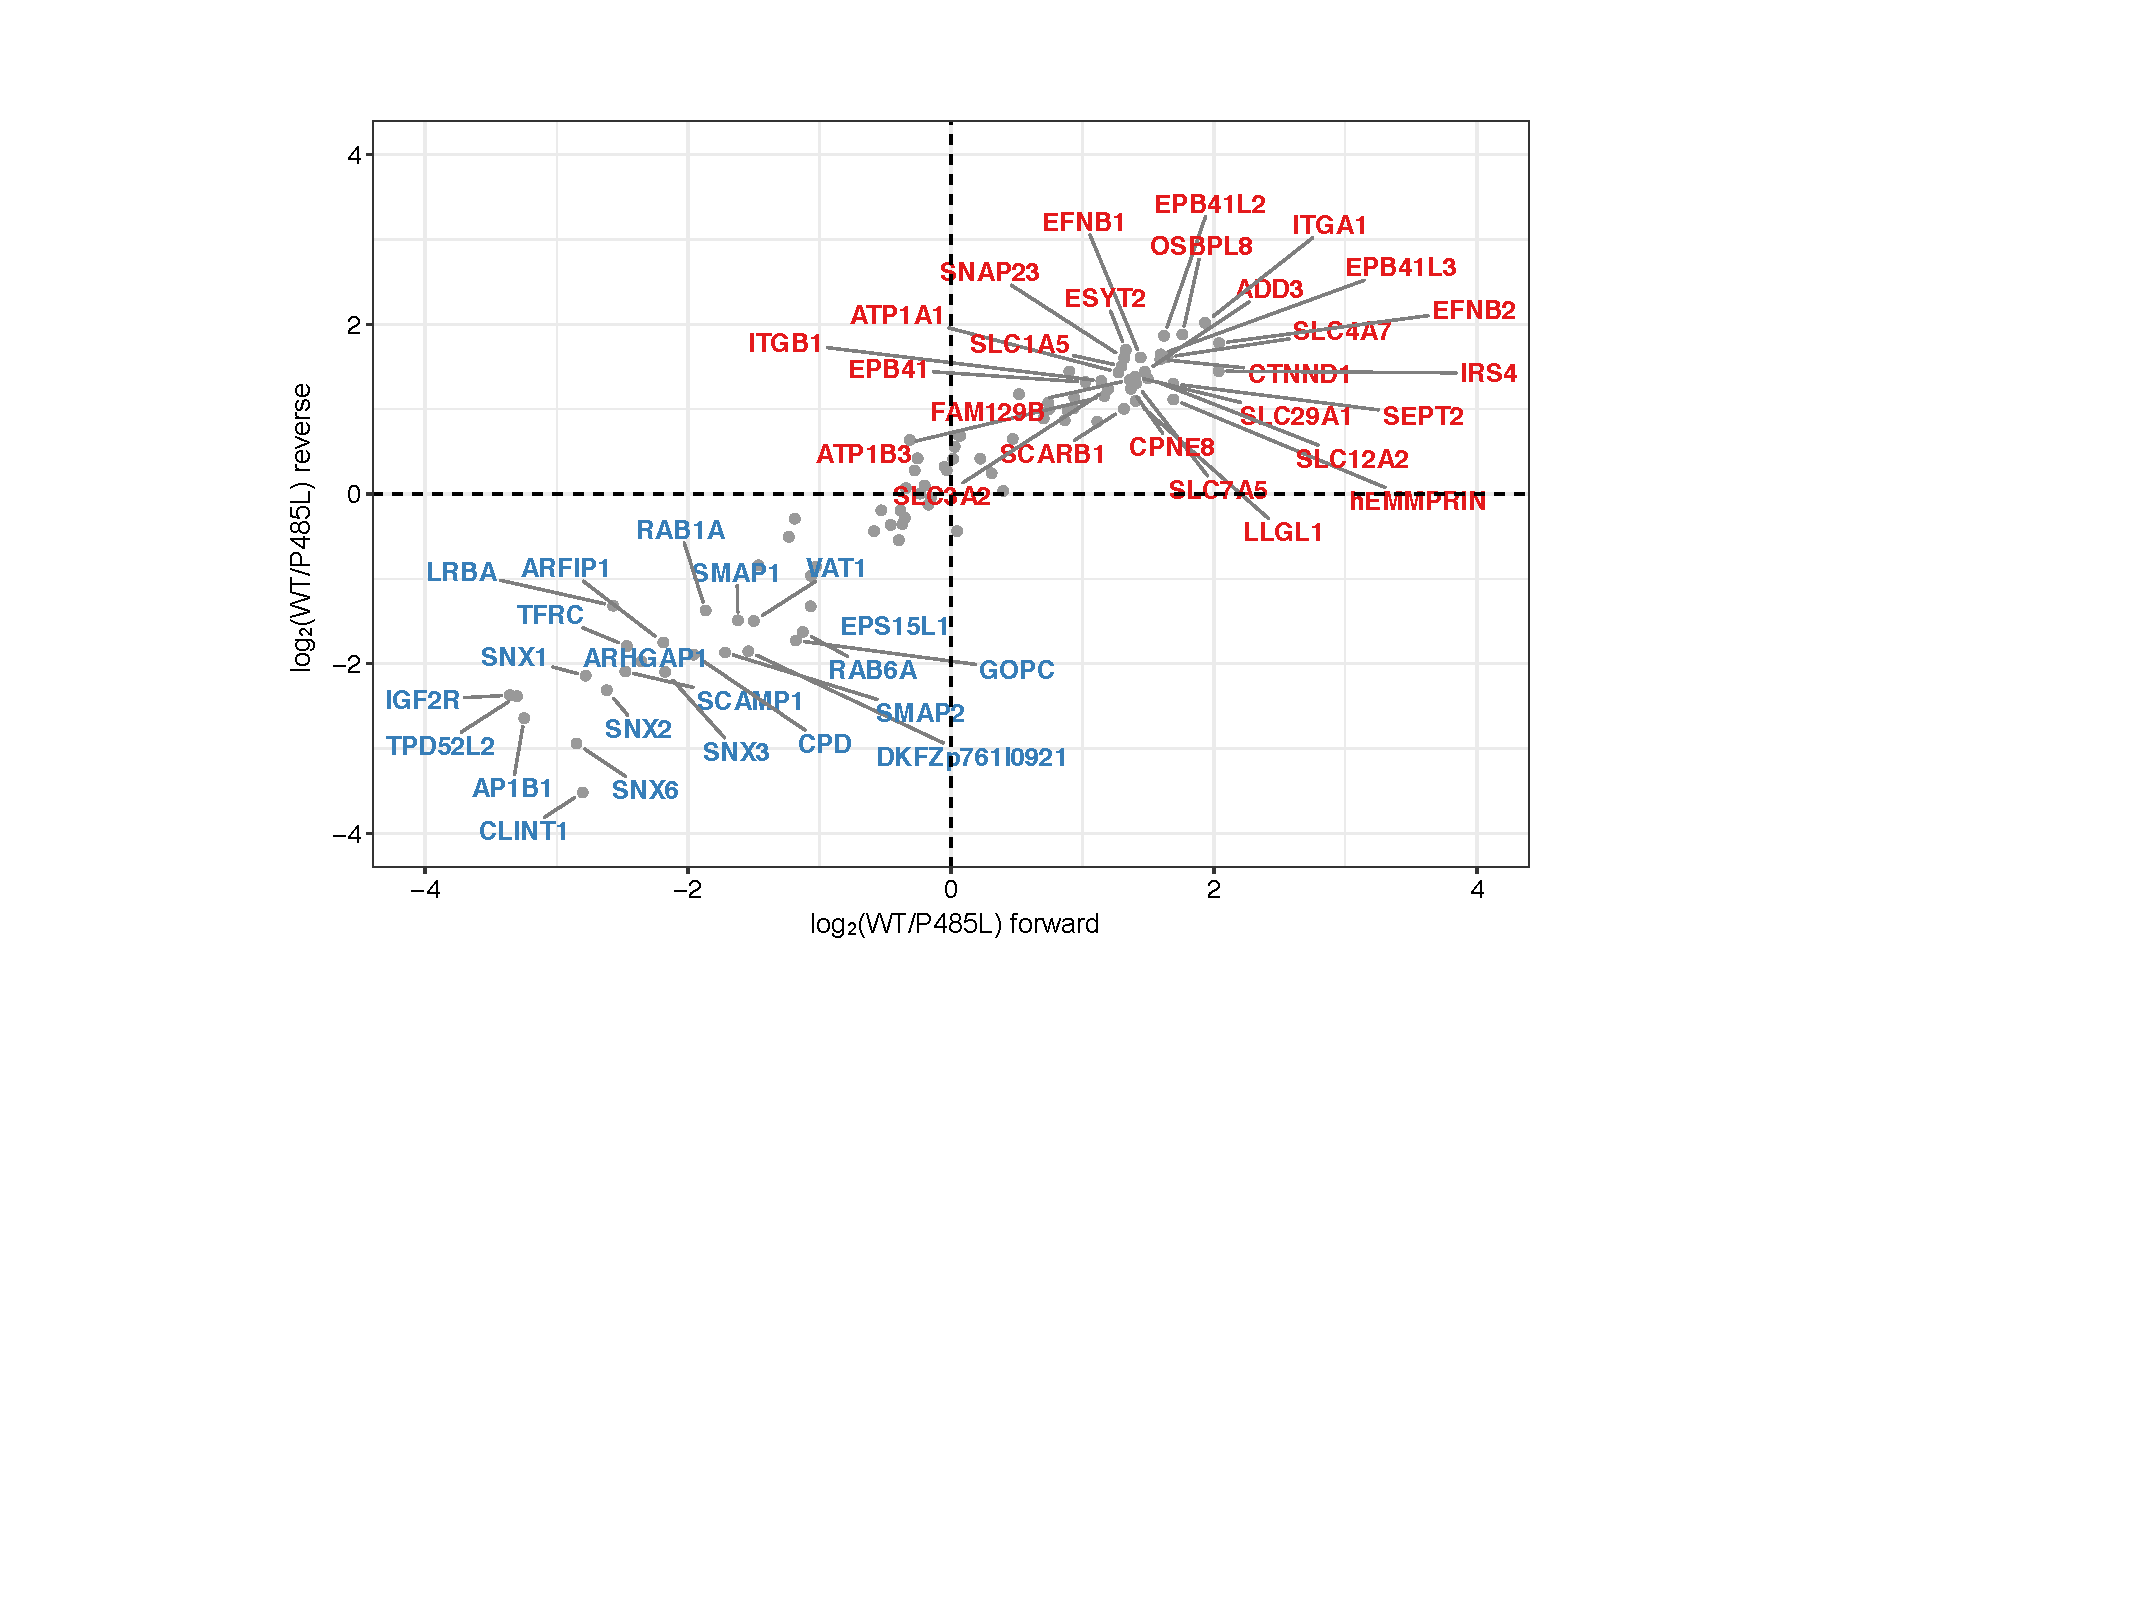
\includegraphics[scale=0.7]{Figures/bioid2}
\caption{SILAC ratio of proteins proximal to the GLUT1 variants.}
\vspace*{-3mm}
\small \justify
HEK293 stable cells expressing GFP1-10 were fully labeled in light (L) isotope medium, whereas HEK293 stable cells expressing BirA-FLAG-GLUT1 wild-type (WT) and BirA-FLAG-GLUT1 mutant (P485L) were fully labeled in medium-heavy (M) or heavy (H) isotope media. The cells were incubated in 0.1 \textmu g/mL doxycycline and 1 mM biotin for 24 hr before being harvested. Purified proteins were quantified by MS/MS analysis. Proteins with a log\textsubscript{2}(H/L) or log\textsubscript{2}(M/L) SILAC ratio smaller than 0.585 (fold change smaller than 1.5) were considered to be background proteins and discarded. After background subtraction, proteins with a log\textsubscript{2}(WT/P485L) or log\textsubscript{2}(P485L/WT) SILAC ratio higher than 1 (fold change larger than 2) in both forward and reverse experiments were identified as specific proximal proteins and the gene names were annotated in red and blue, respectively.
\label{fig:bioid2}
\end{figure}

%Moreover, some of the other proteins identified to be proximal to wild-type GLUT1 have been reported
Conversely, many proteins involved in intracellular trafficking were identified to be proximal to the mutant GLUT1 (Figure~\ref{fig:bioid2}), including sorting nexins (SNX1, SNX2, SNX3) which are components of the retromer complex mediating the retrograde transport from endosomes to the trans-Golgi network~\cite{Rojas,Carlton,Mari,Harterink}. CLINT1, the protein with high mutant/wild-type ratios in both forward and reverse experiments, has been suggested to participate in the transport of cargo proteins via clathrin-coated vesicles from the trans-Golgi network to endosomes~\cite{Mills,Kalthoff,Hirst}. Moreover, IGF2R and TRFC, two receptors identified as proximal proteins of the mutant GLUT1, have been reported to mediate the intracellular trafficking of their corresponding ligands via clathrin-coated vesicles. IGF2R transports lysosomal enzymes from the trans-Golgi network and the cell surface to lysosomes, whereas TRFC is responsible for the internalization of transferrin and its recycling back to the cell surface~\cite{Byrd,Daro}. 
% Together, these data confirmed the differential localization of the wild-type and mutant GLUT1 observed in immunofluorescence microscopy and further indicated that the mutant GLUT1 might reside in clathrin-coated vesicles, several endosomal compartments and the trans-Golgi network.
%At steady state, GLUT1 is localized at the plasma membrane from where it undergoes continuous rounds of endocytosis and PDZ-motif-dependent endosome-to-plasma-membrane recycling (Wieman et al., 2009), the latter being mediated by the SNX27?retromer (Steinberg et al., 2013). RNA interference (RNAi)-mediated suppression of SNX27 or the retromer CSC component VPS35 leads to a pronounced decrease in the amount of GLUT1 at the cell surface and a corresponding decrease in whole-cell levels, as the transporter undergoes missorting and enhanced degradation in the lysosome (Steinberg et al., 2013).

\begin{figure}[h]
\centering
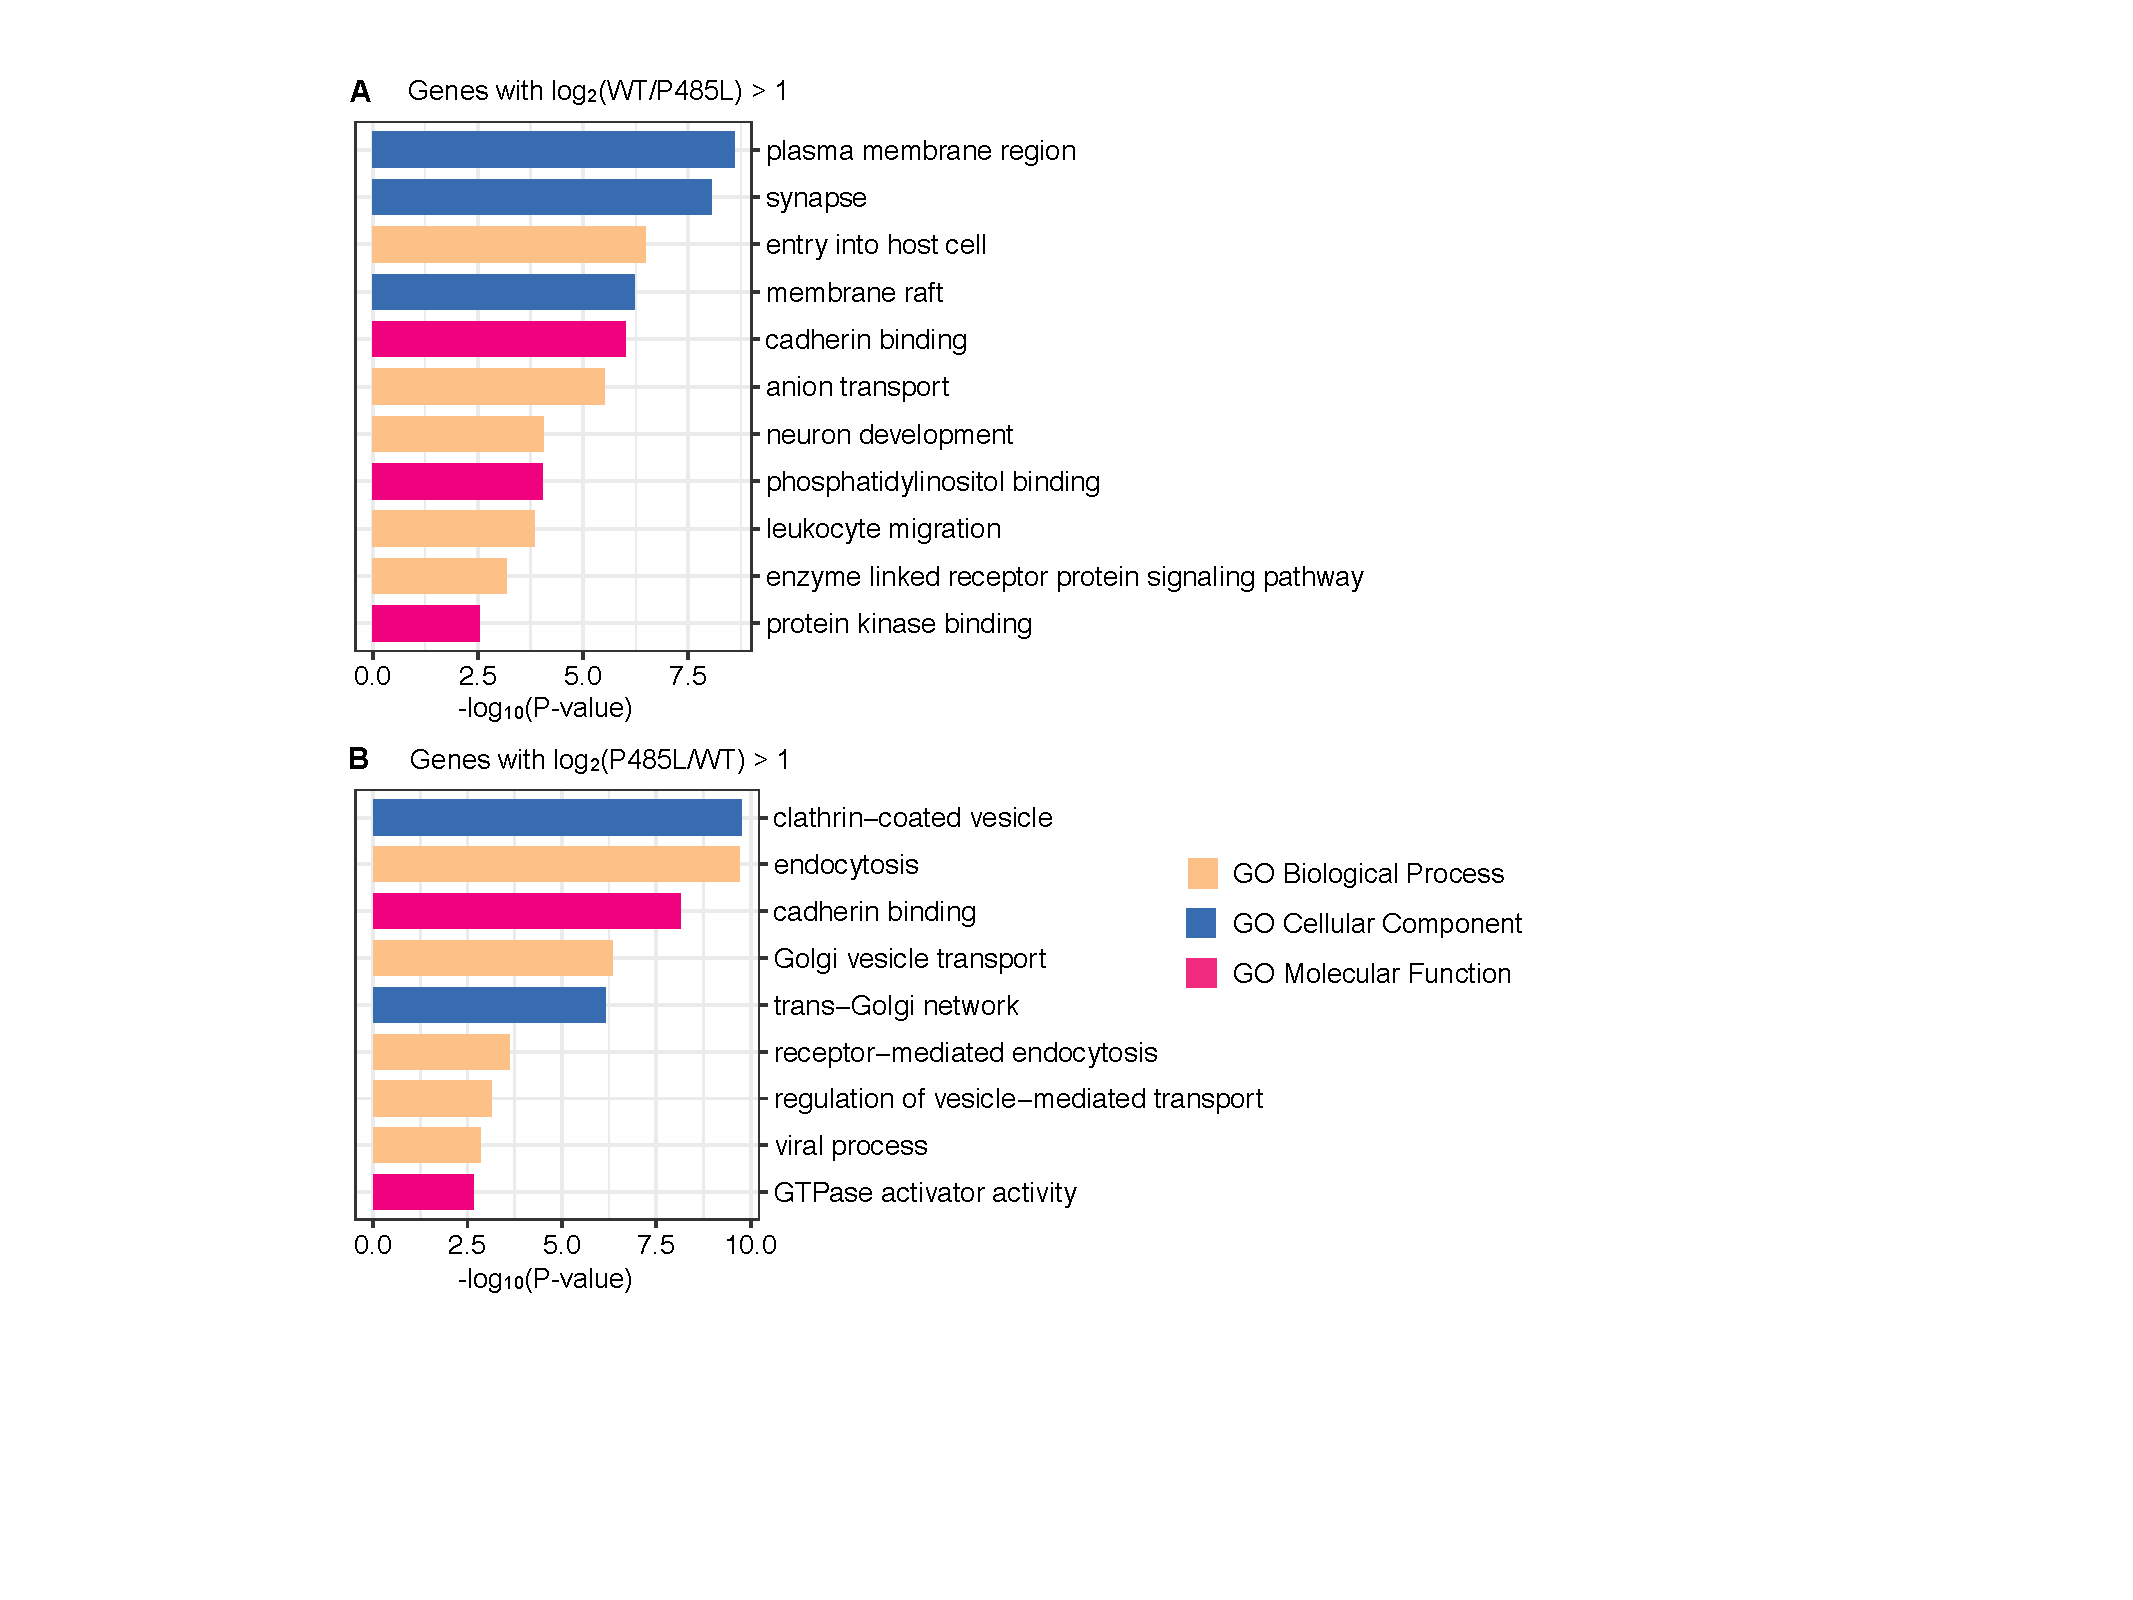
\includegraphics[scale=0.7]{Figures/GO}
\caption{Gene ontology enrichment analysis of GLUT1-proximal proteins.}
\vspace*{-3mm}
\small \justify
Gene ontology analysis was performed with Metascape~\cite{Tripathi}. Only proteins with SILAC H/L and M/L ratios larger than 1.5, WT/P485L ratios larger than 2 in both forward and reverse experiments were selected for the analysis of wild-type specific proteins (A); the analysis of mutant-specific proteins (B) only included proteins with SILAC H/L and M/L ratios larger than 1.5, P485L/WT ratios larger than 2.
\label{fig:go}
\end{figure}
Furthermore, gene ontology (cellular component) analysis of the annotated proteins in Figure~\ref{fig:bioid2} also showed that proteins colocalizing with the wild-type GLUT1 were enriched for plasma membrane proteins ($P=5.89\times 10^{-9}$). In contrast, proteins colocalizing with the mutant GLUT1 were more associated with clathrin-coated vesicles ($P=6.17\times 10^{-10}$), endosomes ($P=2.14\times 10^{-7}$) and retromer complexes ($P=2.45\times 10^{-7}$). Endocytosis was also identified as a significantly enriched biological process in the proteins colocalizing with the mutant GLUT1 ($P=4.27\times 10^{-11}$) (Figure~\ref{fig:go}).

Together, these data confirmed the differential localization of the wild-type and mutant GLUT1 observed in immunofluorescence microscopy and indicated that the GLUT1\textsuperscript{P485L} mutation causes the internalization of the protein via clathrin-dependent endocytosis. Consequently, the mutant protein might reside in clathrin-coated endocytic vesicles, endosomal compartments and the trans-Golgi network.
\section{Co-localization study of GLUT1 variants}
To confirm that the mutant GLUT1 is taken up via clathrin-mediated endocytosis, doxycycline-induced cells were incubated with fluorescently-labeled transferrin (Tf), a known marker for clathrin-mediated endocytosis, and immunostained with the antibody against FLAG~\cite{Hanover}. As expected, extensive colocalization of endocytosed transferrin was detected with the mutant GLUT1, but not with the wild-type GLUT1 (Figure~\ref{fig:tf} C and F).
\begin{figure}[h]
\centering
\includegraphics[scale=0.7]{Figures/tf}
\caption{The mutant GLUT1 co-localizes with endocytosed transferrin.}
\vspace*{-3mm}
\small \justify
Wild-type (WT) and mutant (P485L) GLUT1-expressing cells were cultured on coverslips and induced with 0.1 \textmu g/mL doxycycline for 24 hr. The cells were then incubated with Alexa 568-conjugated transferrin (red, shown in greyscale in B and E) for 10 min before being fixed. The GLUT1 was stained with mouse anti-FLAG and Alexa 488-conjugated anti-mouse antibodies (green, shown in greyscale in A and D). Yellow in the overlay channels (C and F) indicates colocalization of green and red staining. Scale = 10 \textmu m.
\label{fig:tf}
\end{figure}
\begin{figure}[h]
\centering
\includegraphics[scale=0.7]{Figures/EE}
\caption{A subset of the mutant GLUT1 colocalizes with early endosomal markers.}
\vspace*{-3mm}
\small \justify
Wild-type (WT, A-F) and mutant (P485L, G-L) GLUT1-expressing cells were induced with doxycycline and then stained for GLUT1 with mouse anti-FLAG and Alexa 488-conjugated anti-mouse antibodies (green). EEA1 (A-C, G-I) and Rab5 (D-F, J-L) were stained with their corresponding rabbit monoclonal antibodies (Table~\ref{tab:IF}) and Alexa 568-conjugated anti-rabbit antibodies (red). Scale = 10 \textmu m.
%The Rab5 co-staining images were taken with zoom 3 and cropped into the size as shown. 
\label{fig:ee}
\end{figure}

To further determine the subcellular localization of the mutant GLUT1, the GLUT1 expressing cells were co-immunostained with antibodies against organelle-specific marker proteins, including markers for early endosomes, recycling endosomes, late endosomes and the trans-Golgi network. The wild-type GLUT1 showed no colocalization with EEA1 and Rab5, two markers for early endosomes (Figure~\ref{fig:ee} C and I)~\cite{Mu}. By contrast, extensive colocalization was observed between the mutant GLUT1 and the early endosomal markers (Figure~\ref{fig:ee} F and L). Rab5 is a small GTPase involved in the formation of clathrin-coated vesicles (CCV) at the plasma membrane, their subsequent fusion with early endosomes, and the fusion between early endosomes, whereas EEA1 is one of the effector proteins of Rab5 and is recruited selectively on the membrane of early endosomes~\cite{Christoforidis,Rubino,Ballmer}. Because the endocytic CCV is devoid of EEA1, the staining patterns produced by antibodies to EEA1 and Rab5 were not identical (Figure~\ref{fig:ee} B, E, H and K)~\cite{Ballmer}. 
%Some colocalization was observed between Rab5 and the mutant GLUT1, however, the images for this co-staining experiment was taken with a lower resolution than other images, thus were excluded for quantitative colocalization analysis.

\begin{figure}[h]
\centering
\includegraphics[scale=0.7]{Figures/re}
\caption{The mutant GLUT1 does not colocalize with recycling endosomal markers.}
\vspace*{-3mm}
\small \justify
Cells expressing FLAG-tagged wild-type (WT) and mutant (P485L) GLUT1 were co-immunostained with antibodies against FLAG (green) and recycling endosomal markers (red), namely Rab4 (A-C, G-I) and Rab11 (D-F, J-L). Scale = 10 \textmu m.
\label{fig:re}
\end{figure}
We then asked whether the mutant GLUT1 follows the same endosomal recycling as transferrin. Antibodies against two Rab proteins implicated in two distinct recycling pathways, Rab4 and Rab11, were used for this purpose. Rab4 plays a role in fast recycling from early endosomes back to the plasma membrane, whereas Rab11 is a marker for the slow recycling pathway from early endosomes to recycling endosomes, and finally back to the plasma membrane~\cite{Grant}. The mutant GLUT1 did not colocalize with Rab4 or Rab11 (Figure~\ref{fig:re} I and L). It is worth noting that both Rab11 and the wild-type GLUT1 showed staining on the cell surface (Figure~\ref{fig:re} C and F), which is consistent with their respective functional roles. 

\begin{figure}[h]
\centering
\begin{subfigure}[h]{\linewidth}
	\includegraphics[scale=0.7]{Figures/le}
	\label{fig:le1}
	\vspace*{-3mm}
	\small \justify
	\centering (Continued on the next page.)
\end{subfigure}
\end{figure}
\begin{figure}[h]\ContinuedFloat
\centering
\begin{subfigure}[h]{\linewidth}
	\includegraphics[scale=0.7]{Figures/le2}
	\label{fig:le2}
\end{subfigure}
\caption{The mutant GLUT1 colocalizes with Rab9.}
\vspace*{-3mm}
\small \justify
Cells expressing FLAG-tagged wild-type (WT) and mutant (P485L) GLUT1 were co-immunostained with antibodies against FLAG (green) and late endosomal markers (red), namely Rab9 (A-C, J-L), Rab7 (D-F, M-O) and LAMP1 (G-I, P-R). Scale = 10 \textmu m.
\label{fig:le}
\end{figure}
Having shown that the mutant GLUT1 is not a cargo for endosomal recycling, we next investigated whether it is located in late endosomes and targeted for lysosomal degradation. Three different late endosomal markers were used for the colocalization analysis: Rab9 mediates trafficking from late endosomes to the trans-Golgi network, Rab7 mediates trafficking from late endosomes to lysosomes, and LAMP1 is associated with endo-lysosomal structures~\cite{Stenmark,Saftig}. As expected, the wild-type GLUT1 did not colocalize with the late endosomal markers (Figure~\ref{fig:le} C, F and I). Interestingly, the mutant GLUT1 did not show significiant colocalization with Rab7 or LAMP1 either (Figure~\ref{fig:le} O and R), suggesting that the lysosomal degradation pathway might not be a major part of the mutant GLUT1 trafficking. However, the mutant GLUT1 did show significant tendency to colocalize with Rab9 (Figure~\ref{fig:le} L), indicating that a great proportion of endocytosed mutant GLUT1 might reside in the trans-Golgi network.
% A great proportion of endocytosed mutant GLUT1 was contained in Rab9-positive endosomes.
\begin{figure}[h]
\centering
\includegraphics[scale=0.7]{Figures/tgn}
\caption{The mutant GLUT1 co-localizes with TGN markers.}
\vspace*{-3mm}
\small \justify
Cells expressing FLAG-tagged wild-type (WT) and mutant (P485L) GLUT1 were co-immunostained with antibodies against FLAG (green) and markers for the trans-Golgi network (TGN, red), namely Vti1a (A-C, G-I) and Vti1b (D-F, J-L). Scale = 10 \textmu m.
\label{fig:tgn}
\end{figure}

Through the recruitment of specific effector proteins, the Rab GTPases regulate intracellular trafficking processes such as membrane recruitment and membrane fusion~\cite{Stenmark}. As the other key component of the intracellular trafficking apparatus, the SNARE complexes are principal effectors of membrane fusion by forming tetrahelical bundles~\cite{Stenmark,Chen,Ohya}. Two SNARE proteins with distinct but overlapping localization, Vti1a and Vti1b, were used as markers for Golgi-associated trafficking to study the subcellular localization of the mutant GLUT1. Localized at the trans-Golgi network, Vti1a mediates the receipt of cargoes from early endosomes (Rab9-independent) and late endosomes (Rab9-dependent)~\cite{Ganley}. Vti1b is predominantly localized on tubules and vesicles in the trans-Golgi area and on late endosomes, where it has been shown to mediate the fusion of late endosomes together and with lysosomes~\cite{Kreykenbohm,Antonin,Pryor}. In contrast to the distinct localization of the wild-type GLUT1 and Golgi markers, the mutant GLUT1 showed extensive colocalization with both markers (Figure~\ref{fig:le} C, F, I and L), thereby confirming that the mutant GLUT1 is localized to the trans-Golgi network.
%To confirm this, the colocalization of GLUT1 and trans-Golgi markers was analyzed. 
%colocalize at the perinuclear region

Finally, the colocalization of GLUT1 variants and co-immunostaining markers was quantified by 
%processing the images with the software Imaris and 
measuring Pearson's thresholded colocalization coefficents in three-dimensional images with voxel size consistent with the Nyquist criterion~\cite{Costes,Webb}. The co-immunostaining images for FLAG and Rab5 (Figure~\ref{fig:ee} F and L) were excluded from quantitative analysis because the resolutions were not optimal. Because of time constraints, analysis based on replicate images was only performed on 7 pairs of proteins, and the analysis for the rest 11 pairs of proteins did not include biological replicates. However, the regions for image aquisition were selected by viewing nuclear (DAPI) staining, and the analysis for each staining included at least three cells, therefore human bias and noise were reduced in the datasets used for colocalization analysis. As shown in Figure~\ref{fig:coloc}, transferrin, Rab9, Vti1a and Vti1b showed high tendency to colocalize with the mutant GLUT1, indicating that the endocytosed mutant GLUT1 might be largely localized in early endosomes, late endosomes and the trans-Golgi network.
\begin{figure}[h]
\centering
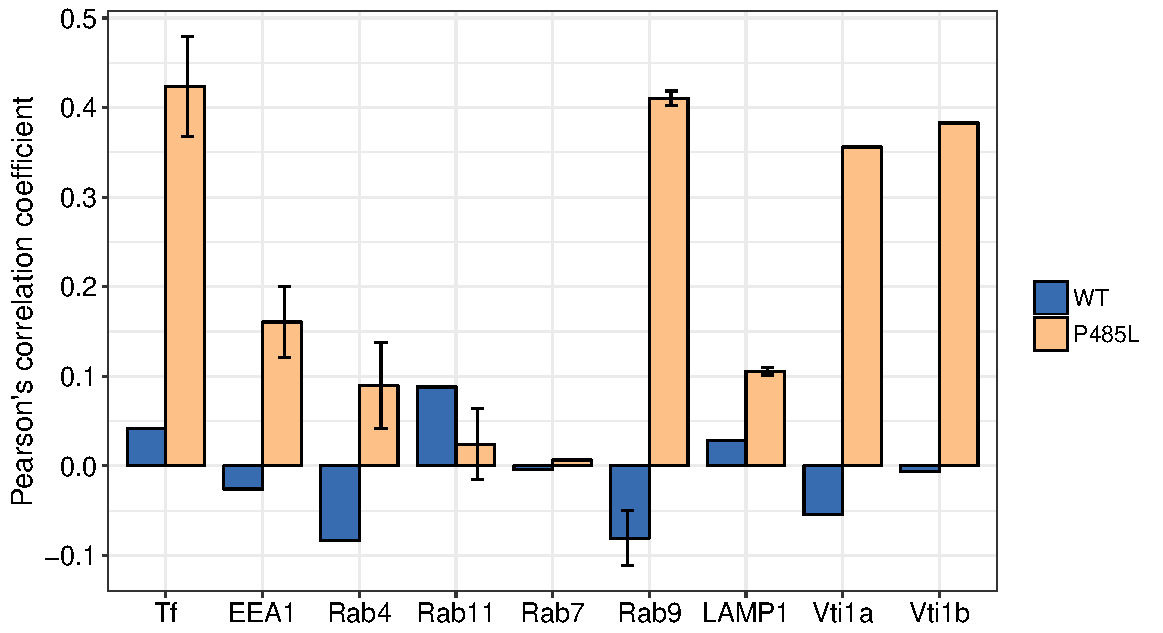
\includegraphics[scale=0.7]{Figures/coloc}
\caption{Colocalization coefficients for GLUT1 variants and intracellular markers.}
\vspace*{-3mm}
\small \justify
Pearson's thresholded coefficients (as implemented in the Imaris software) was determined for the indicated pairs of proteins. Three z-stack images from biological replicates were evaluated for the colocalization of the mutant GLUT1 and Rab9/LAMP1, and the wild-type GLUT1 and Rab9, whereas two images were evaluated for the colocalization of the mutant GLUT1 and transferrin/EEA1/Rab4/Rab11. For these analyses, mean values were expressed with standard deviations of the mean.
\label{fig:coloc}
\end{figure}
%----------------------------------------------------------------------------------------
% Define some commands to keep the formatting separated from the content 

% Chapter 4

\chapter{Discussion} % Main chapter title
\label{Chapter4} % For referencing the chapter elsewhere, use \ref{Chapter4} 
\addtocontents{toc}{\setcounter{tocdepth}{1}}
GLUT1 serves as the primary glucose transporter across vascular endothelial cells of the human blood-brain barrier~\cite{Pascual}. Mutations in GLUT1 can cause impaired glucose transport into the brain, leading to G1DS~\cite{Klepper.2}. A new GLUT1 mutation, GLUT1\textsuperscript{P485L}, was reported in 2009 in a child with G1DS, but its pathogenic mechanisms remain unknown~\cite{Slaughter}.

In a recent study by our group, a novel interaction was discovered between a short peptide in the carboxyl terminal of GLUT1 carrying the P485L mutation and clathrin, but this interaction is absent in the binding profile of the corresponding wild-type peptide~\cite{Meyer2}. Furthermore, sequence analysis revealed that the mutation creates a novel short linear motif ([DE]XXXL[LI]) that is known to mediate endocytosis and intracellular trafficking of membrane proteins~\cite{Meyer2,Bonifacino}. In HeLa cells transiently transfected with GLUT1, the wild-type GLUT1 was localized to the plasma membrane, whereas the mutant GLUT1 showed vesicular localization and colocalization with endocytosed transferrin~\cite{Meyer2}. Moreover, BioID experiments in HEK293 cells with GLUT1 transient expression showed increased colocalization of the mutant GLUT1 with proteins associated with clathrin-mediated endocytosis and endosomal trafficking~\cite{Meyer2}. These results suggested that the GLUT1\textsuperscript{P485L} mutation causes internalization of the protein via clathrin-mediated endocytosis~\cite{Meyer2}. 

In this thesis, we used two HEK293 stable cell lines with stable inducible GLUT1 expression to further investigate the effect of the GLUT1\textsuperscript{P485L} mutation on the intracellular localization and trafficking of the protein.

\section{Subcellular localization of GLUT1}
In agreement with previous observations in HeLa cells transiently transfected with GLUT1, confocal images of GLUT1 localization in HEK293 cells stably expressing FLAG-GLUT1 confirmed the mislocalization of the mutant GLUT1 in intracellular vesicles~\cite{Meyer2}. Furthermore, the mutant GLUT1 showed colocalization with early endosomal markers (EEA1, Rab5), a late endosomal marker (Rab9), and markers for the trans-Golgi network (Vti1a, Vti1b).
% Rab7, LAMP1
% quantification
% bioid
%\section{Intracellular trafficking of GLUT1}
% motif
\section{Leakiness and loss of GLUT1 expression}
%When culturing cells in medium containing fetal bovine serum (FBS), please note that many lots of FBS contain tetracycline as FBS is generally isolated from cows that have been fed a diet containing tetracycline. If you culture your cells in medium containing FBS that is not reduced in tetracycline, you may observe low basal expression of your gene of interest in the absence of tetracycline

%Tetracycline (MW = 444.4) is commonly used as a broad spectrum antibiotic and acts to inhibit translation by blocking polypeptide chain elongation in bacteria. In the T-REx? System, tetracycline is used as an inducing agent to induce transcription of the gene of interest from the inducible expression vector. Tetracycline induces transcription by binding to the Tet repressor homodimer and causing the repressor to undergo a conformational change that renders it unable to bind to the Tet operator. The association constant of tetracycline to the Tet repressor is 3 x 109 M-1 (Takahashi et al., 1991). 

%Tetracycline is light sensitive

%You may want to vary the concentration of tetracycline (0.1 to 1 �g/ml) and time of exposure to tetracycline (8 to 24 hours) to optimize or modulate expression for your cell line.

%Stable cell lines often lose their protein expression with time as a result of a heterogeneity in the transfected population of cells. A more homogeneous population of cells can be obtained by limiting dilution cloning or picking individual colonies of drug-resistant cells.

% selection used by the landhaler lab; one population might overgrow another, causing the increased leaky expression over time.

Because the loss of expression over time was observed in a sub-population of both wild-type and mutant cells (Figure%figure! 
, new cells were thaw and the expression of GLUT1 variants were analyzed again with Western blotting and immunofluorescence microscopy. (Supplementary Figure%figure!

\section{Conclusion and outlook}
%----------------------------------------------------------------------------------------
% Define some commands to keep the formatting separated from the content 
 
%\include{Chapters/Chapter5} 

%----------------------------------------------------------------------------------------
%	ABBREVIATIONS
%----------------------------------------------------------------------------------------

\begin{abbreviations}{ll} % Include a list of abbreviations (a table of two columns)
\addchaptertocentry{\abbrevname}
\textbf{ABC} & Ammonium bicarbonate\\
\textbf{AGC} & Automatic gain control\\
\textbf{AP} & Adaptor protein\\
\textbf{BAF} & Bafilomycin A1\\
\textbf{BioID} & Proximity-dependent biotin identification\\
\textbf{BSA} & Bovine serum albumin\\
\textbf{CCV} & Clathrin-coated vesicle\\
\textbf{CSF} & Cerebrospinal fluid\\
\textbf{DAPI} & 4',6-Diamidino-2-phenylindole\\
\textbf{DMEM} & Dulbecco's modified Eagle's medium\\
\textbf{DOX} & Doxycycline\\
\textbf{DPSS} & Diode-pumped solid-state\\
\textbf{DTT} & Dithiothreitol\\
\textbf{EDTA} & Ethylenediaminetetraacetic acid\\
\textbf{EEA1} & Early endosome antigen 1\\
\textbf{GAP} & GTPase-activating protein\\
\textbf{GFP} & Green fluorescent protein\\
\textbf{GLUT1} & Facilitated glucose transporter member 1\\
\textbf{GO} & Gene ontology\\
\textbf{G1DS} & Glucose transporter 1 deficiency syndrome\\
\textbf{H} & Heavy\\
\textbf{HCMV} & Human cytomegalovirus\\
\textbf{HEK293} & Human embryonic kidney 293\\
\textbf{HEPES} & 4-(2-Hydroxyethyl)-1-piperazineethanesulfonic acid)\\
\textbf{HPLC} & High-pressure liquid chromatography\\
\textbf{hr} & Hour\\
\textbf{HRP} & Horseradish peroxidase\\
\textbf{IAA} & Iodoacemtamide\\
\textbf{L} & Light\\
\textbf{IgG} & Immunoglobulin G\\
\textbf{LAMP1} & Lysosomal-associated membrane protein 1\\
\textbf{LC3} & Microtubule-associated protein 1A/1B-light chain 3\\
\textbf{M} & Medium-heavy\\
\textbf{MNK} & Menkes protein\\
\textbf{MS} & Mass spectrometry\\
\textbf{MS/MS} & Tandem mass spectrometry\\
\textbf{PBS} & Phosphate-buffered saline\\
\textbf{PCR} & Polymerase cain reaction\\
\textbf{PFA} & Paraformaldehyde\\
\textbf{PMT} & Photomultiplier tube\\
\textbf{PVDF} & Polyvinylidene fluoride\\
\textbf{rcf} & Relative centrifugal force\\
\textbf{RIPA} & Radioimmunoprecipitation assay\\
\textbf{rpm} & Revolutions per minute\\
\textbf{SDS-PAGE} & Sodium dodecyl sulfate polyacrylamide gel electrophoresis\\
\textbf{SILAC} & Stable isotope labeling by amino acids in cell culture\\
\textbf{SLC} & Solute carrier\\
\textbf{SNARE} & Soluble N-ethylmaleimide-sensitive fusion protein-attachment protein receptor\\
\textbf{SNX} & Sorting nexin\\
\textbf{STX6} & Syntaxin 6\\
\textbf{TAP} & Tandem affinity purification\\
\textbf{TBST} & Tris buffered saline with Tween 20\\
\textbf{Tet} & Tetracycline\\
\textbf{TetR} & Tetracycline repressor\\
\textbf{Tf} & Transferrin\\
\textbf{TFA} & Trifluoroacetic acid\\
\textbf{TGN} & Trans-Golgi network\\
\textbf{TRFC} & Transferrin receptor\\
\textbf{tris} & Tris(hydroxymethyl)aminomethane\\
\textbf{WT} & Wild-type\\

\end{abbreviations}

%----------------------------------------------------------------------------------------
%	ACKNOWLEDGEMENTS
%----------------------------------------------------------------------------------------

\begin{acknowledgements}
\addchaptertocentry{\acknowledgementname} % Add the acknowledgements to the table of contents
This study was carried out in the Protein Dynamics Laboratory at Max Delbr\"{u}ck C	enter of Molecular Medicine. I would like to thank Professor Matthias Selbach for having given me the opportunity to complete my Master's thesis in his laboratory. I am also very grateful to my thesis supervisor Katrina Meyer who introduced me to this extraordinarily interesting project and offered me continuous support throughout the thesis. Her guidance and encouragement has been most inspiring and invaluable.

I would also like to thank Ouidad Benlasfer from the the laboratory of Professor Markus Landthaler for kindly providing the HEK293 stable cell lines. Additionally, I want to thank Giulia Russo from the department of Professor Volker Haucke for her help with immunofluorescence assays. For their great work and technical support I am very thankful to the Advanced Light Microscopy technology platform at MDC. Special thanks to Konstantin Grohmann for helping me with the colocalization analyses.

I would very much like to thank all the members of the lab. I have always felt welcome to ask for any help and support that I needed. I would like to express my special regards to Jo\~{a}o Fernandes, Dr.\ Michal Nadler-Holly, Dr.\ Matthias Ziehm and Martha Hergeselle for the inspiring and supportive discussions in the SBTH office. Alongside, I also thank Dr.\ Koshi Imami, Christian Sommer and the rest of the group members for providing a most pleasant working environment.

I want to thank my friends from the MolMed program and Tsinghua University for all the necessary distractions and laughters. I must thank our three cats, Salph, Twrx and Princess, who have always cheered me up with magic when I had difficulties. Finally, my deepest gratitude goes to my boyfriend Nimo, his and my family for understanding and encouraging me throughout the time it took to finish the present work.

\end{acknowledgements}

%----------------------------------------------------------------------------------------
%	THESIS CONTENT - APPENDICES
%----------------------------------------------------------------------------------------

%\appendix % Cue to tell LaTeX that the following "chapters" are Appendices

% Include the appendices of the thesis as separate files from the Appendices folder
% Uncomment the lines as you write the Appendices

%% Appendix A

\chapter{Frequently Asked Questions} % Main appendix title

\label{AppendixA} % For referencing this appendix elsewhere, use \ref{AppendixA}

\section{How do I change the colors of links?}

The color of links can be changed to your liking using:

{\small\verb!\hypersetup{urlcolor=red}!}, or

{\small\verb!\hypersetup{citecolor=green}!}, or

{\small\verb!\hypersetup{allcolor=blue}!}.

\noindent If you want to completely hide the links, you can use:

{\small\verb!\hypersetup{allcolors=.}!}, or even better: 

{\small\verb!\hypersetup{hidelinks}!}.

\noindent If you want to have obvious links in the PDF but not the printed text, use:

{\small\verb!\hypersetup{colorlinks=false}!}.

%\include{Appendices/AppendixB}
%\include{Appendices/AppendixC}

%----------------------------------------------------------------------------------------
%	BIBLIOGRAPHY
%----------------------------------------------------------------------------------------
\begin{Literature}
\addchaptertocentry{\literaturename} 
\nocite{apsrev41Control}
\bibliography{main,revtex-custom}
\end{Literature}

%----------------------------------------------------------------------------------------
\begin{statement}
\addchaptertocentry{\statementname}
\vspace{10pt}
Herewith I confirm that I wrote this Master's Thesis in its entirety and that no additional assistance was provided, other than from the sources listed.
\end{statement}

\end{document}  
